% Template para uso no TCC do Departamento de F�sica de Ji-Paran�
% da Universidade Federal de Rond�nia
% Elaborado em 10 de junho de 2017 por Marco Polo Moreno de Souza com base no template book.
% Aperfei�oado em 07 de mar�o de 2019, com a introdu��o de macros
% Modifica��o na estrutura do de oneside para twoside 1 de setembro de 2019
%Resolu��o de warning.

\documentclass[a4paper,reqno,12pt,twoside]{book}
\small
\RequirePackage{fix-cm}
\usepackage{amsmath}%
\usepackage{amsfonts}%
\usepackage{amssymb}%
%\usepackage{graphicx}%
\usepackage{physics}%
\usepackage{blindtext}
\usepackage
[ruled, % Caixa em volta, leg. acima, linha ap�s leg.
portuguese] % Para algoritmos em portugu�s.
{algorithm2e} % Enfim o pacote.
%Veja o arquivo abaixo antes de adicionar outras bibliotecas
\usepackage[mode=buildnew]{standalone}% requires -shell-escape

\usepackage[imagemagick]{sagetex}

\usepackage{calc}
%\usepackage{svg}
\usepackage{pst-text}
\newcommand{\executeiffilenewer}[3]{%
	\ifnum\pdfstrcmp{\pdffilemoddate{#1}}%
	{\pdffilemoddate{#2}}>0%
	{\immediate\write18{#3}}\fi%
}
\newcommand{\includesvg}[1]{%
	\executeiffilenewer{#1.svg}{#1.pdf}%
	{inkscape -z -D --file=#1.svg %
		--export-pdf=#1.pdf --export-latex}%
	\input{#1.pdf_tex}%
}
\usepackage{cancel}
\usepackage{scrextend}
%\usepackage{indentfirst}
\usepackage{float}
\usepackage[brazilian]{babel}
\usepackage[latin1]{inputenc}
\usepackage{times}
\usepackage[T1]{fontenc}
\usepackage[final]{pdfpages}
\usepackage{epstopdf}
\usepackage[top=3cm,bottom=2cm,left=3cm,right=2cm,marginparsep=0pt]{geometry}
\usepackage{multirow}
\usepackage[colorlinks=true,linkcolor=blue,citecolor=red,urlcolor=black,bookmarks=true,pdfstartview=FitB]{hyperref} %uso de links
%\usepackage[hyphenbreaks]{breakurl}
%\usepackage{makeidx}
%\makeindex
\usepackage{wrapfig}
\usepackage{flashmovie}
\usepackage{fancyhdr} %cabe�alho
\usepackage{setspace} %espa�amento entre linhas

\usepackage{titlesec}    
\titleformat{\chapter}[display]
{\normalfont%
	\Large% %change this size to your needs for the first line
	\bfseries}{\chaptertitlename\ \thechapter}{20pt}{%
	\Large %change this size to your needs for the second line
}

\usepackage{xcolor}
\definecolor{verde}{rgb}{0,0.5,0}
\usepackage{showexpl} % exibe codigos de figuras
\usepackage{listings}
\lstset{
	language=C++,
	basicstyle=\ttfamily\small, 
	keywordstyle=\color{blue}, 
	stringstyle=\color{verde}, 
	commentstyle=\color{red}, 
	extendedchars=true, 
	showspaces=false, 
	showstringspaces=false, 
	numbers=left,
	numberstyle=\tiny,
	breaklines=true, 
	backgroundcolor=\color{green!10}, 
	breakautoindent=true, 
	captionpos=b,
	xleftmargin=0pt,
	emph={main, printf, scanf},
	emphstyle={\color{black}\bf},
	morekeywords={comando1, comando2},language=C++,
	basicstyle=\ttfamily\small,
	keywordstyle=\color{blue},
	stringstyle=\color{verde},
	commentstyle=\color{red},
	extendedchars=true,
	showspaces=false,
	showstringspaces=false,
	numbers=left,
	numberstyle=\tiny,
	breaklines=true,
	backgroundcolor=\color{green!10},
	breakautoindent=true,
	captionpos=b,
	xleftmargin=0pt,
}
\usepackage{amsmath}
\usepackage[font=footnotesize, labelfont=bf, margin=0.5cm]{caption} %Altera formata��o das legendas
\usepackage{indentfirst} %Espa�amento aplicado � primeira linha do primeiro par�grafo
%%%%%%%%%%%%%%%%%%%%%%
\usepackage{color}
\usepackage{ifpdf}
\ifpdf %if using pdfLaTeX in PDF mode
%\usepackage[pdftex]{graphicx}
\DeclareGraphicsExtensions{.pdf,.png,.jpg,.jpeg,.mps}
\usepackage{pgf}
\usepackage{tikz}
\else %if using LaTeX or pdfLaTeX in DVI mode
\usepackage{graphicx}
\DeclareGraphicsExtensions{.eps,.bmp}
\DeclareGraphicsRule{.emf}{bmp}{}{}% declare EMF filename extension
\DeclareGraphicsRule{.png}{bmp}{}{}% declare PNG filename extension
\usepackage{pgf}
\usepackage{tikz}
\usepackage{pstricks}
\fi
\usepackage{epic,bez123}
\usepackage{floatflt}% package for floatingfigure environment
\usepackage{wrapfig}% package for wrapfigure environment

%%%%%%%%%%%%%%%

\makeatletter
\newcommand{\showfont}
{%
	(encoding: \f@encoding{},
	family: \f@family{},
	series: \f@series{},
	shape: \f@shape{},
	size: \f@size{},
	baseline: \f@baselineskip{})
	%tfsize: \tf@size{},
	%sfsize: \sf@size{},
	%sssize: \ssf@size{}
}
\makeatother

%%%%%%%%%%%%%%%%%%%%%%%%%%%%%%%%%%%%%%%%%%%%%%%%%%%%%%%%%%%%%%%

%Preencha os campos abaixo conforme seu TCC
\newcommand{\Titulo}{Propaga��o de pulsos de luz em sistemas at�micos}
\newcommand{\Nome}{Eliton Trindade Gomes}
\newcommand{\curso}{Bacharelado} %Digite Licenciatura Plena ou Bacharelado
\newcommand{\graduacao}{Bacharel} %Digite Licenciado ou Bacharel conforme o caso
\newcommand{\orientador}{Dr. Marco Polo Moreno de Souza} %Nome com t�tulo. Ex: Dr. Marco Polo Moreno de Souza
\newcommand{\primeiromembro}{Nome do professor da banca} %Nome com t�tulo. Ex: Dr. Fulano de Tal
\newcommand{\segundomembro}{Nome do professor da banca} %Nome com t�tulo. Ex: MSc. Beltrano
\newcommand{\instituicao}{DEFIJI/CJP/UNIR} %Institui��o do segundo membro. Se for interno, digite DEFIJI/CJP/UNIR
\newcommand{\Cidade}{Ji-Paran�, RO}
\newcommand{\Data}{M�s e ano da defesa}

%%%%%%%%%%%%%%%%%%%%%%%%%%%%%%%%%%%%%%%%%%%%%%%%%%%%%%%%%%%%%%%
%Dados da defesa, a ser preenchido pelo orientador
\newcommand{\dia}{xxx} %Ex: quinze
\newcommand{\mes}{xxx} %Ex: abril
\newcommand{\ano}{xxx} %Ex: 2019
\newcommand{\inicio}{xxx} %In�cio da defesa. Ex: 10:15 h
\newcommand{\fim}{xxx} %Fim da sess�o. Ex: 11:45 h
\newcommand{\arguicao}{xxx} %Dura��o da argui��o da banca em minutos. Ex: 45
\newcommand{\arguicaoextenso}{xxx} %Idem acima, por extenso. Ex: quarenta e cinco
\newcommand{\local}{xxx} %Ex: audit�rio do Campus da UNIR de Ji-Paran�
\newcommand{\nota}{xxx} %Ex: 8,5
\newcommand{\notaextenso}{xxx} %Ex: oito inteiros e cinco d�cimos

\newcommand{\titulo}{\expandafter\MakeUppercase\expandafter{\Titulo}}
\newcommand{\nome}{\expandafter\MakeUppercase\expandafter{\Nome}}
\newcommand{\cidade}{\expandafter\MakeUppercase\expandafter{\Cidade}}
\newcommand{\data}{\expandafter\MakeUppercase\expandafter{\Data}}
\setlength{\headheight}{15pt}
\titleformat{\chapter}
{\normalfont\bfseries}{\thechapter}{0.3em}{\MakeUppercase}
\titlespacing*{\chapter}{0pt}{-36pt}{36pt}

\titleformat{\section}
{\normalfont}{\thesection}{0.3em}{\MakeUppercase}
\titlespacing*{\section}{0pt}{36pt}{36pt}

\titleformat{\subsection}
{\normalfont\bfseries}{\thesubsection}{0.3em}{}
\titlespacing*{\subsection}{0pt}{36pt}{36pt}

\setlength{\parindent}{1.25cm} %Primeira linha do par�grafo
%\renewcommand{\baselinestretch}{1.5} %
%\setstretch{1.5}

%Coloca a numera��o no canto externo da p�gina (necess�rio para impress�o frente e verso)
\pagestyle{fancy}
\fancyhf{}
\renewcommand{\headrulewidth}{0pt}% elimina linhas horizontais
\fancyhead[RO, LE]{\thepage}

%Faz o mesmo que a sequ�ncia acima em p�ginas onde se come�am cap�tulos
\fancypagestyle{plain}{%
	\renewcommand{\headrulewidth}{0pt}%
	\fancyhf{}%
	\fancyhead[RO, LE]{\thepage}
}

\begin{document}
	\pagenumbering{Alph}
	\renewcommand{\bibname}{Refer�ncias}
	\chapter*{}
\thispagestyle{empty}

\vspace{-1cm}
\begin{center}
\textbf{\nome}
\end{center}

\vspace{3.5cm}
\begin{figure}[htbp]
	\centering
		
\includegraphics[width=0.99\textwidth]{logo.eps}
\end{figure}
\vspace{4cm}

\begin{center}
\textbf{\titulo}
\end{center}

\vspace{8cm}
\begin{center}
\textbf{\cidade} \\ \textbf{\data}
\end{center}
	\chapter*{}
\thispagestyle{empty}

\vspace{-1cm}

\begin{center}
\textbf{\nome}
\end{center}

\vspace{11cm}

\begin{center}
\textbf{\titulo}
\end{center}

\vspace{1cm}

\begin{minipage}{0.4\linewidth}
.
\end{minipage}
\begin{minipage}{0.5\linewidth}
Trabalho de Conclus�o de Curso apresentado
ao Departamento de F�sica de Ji-Paran�,
Universidade Federal de Rond�nia, Campus de
Ji-Paran�, como parte dos quesitos para a
obten��o do T�tulo de {\graduacao} em F�sica, sob orienta��o do Prof.
{\orientador}.
\end{minipage}

\vspace{5cm}

\begin{center}
\textbf{\cidade}\\
\textbf{\data}
\end{center}
	\chapter*{}
\thispagestyle{empty}
\vspace{-2cm}

\begin{figure}[htbp]
	\centering
		
\includegraphics[width=0.95\textwidth]{logo-ata.eps}
\end{figure}
\vspace{0.3cm}
\begin{center}
\textbf{ATA DE AVALIA��O DO TRABALHO DE CONCLUS�O DE CURSO DO CURSO DE (LICENCIATURA PLENA/BACHARELADO) EM F�SICA}
\end{center}
\vspace{0.7cm}
\doublespacing

\noindent Aos {\dia} dias do m�s de {\mes} do ano de {\ano}, �s {\inicio}, no {\local}, reuniu-se a Banca Julgadora composta pelo professor orientador {\orientador} e pelos examinadores {\primeiromembro} e {\segundomembro}, para avaliarem o Trabalho de Conclus�o de Curso, do Curso de
{\curso} em F�sica, intitulado ``\textbf{\titulo}'', do discente {\textit{\nome}}. Ap�s a apresenta��o, o candidato foi arguido pelos integrantes da Banca Julgadora por {\arguicao} ({\arguicaoextenso}) minutos. Ao final da argui��o, a Banca Julgadora, em sess�o reservada, \textbf{aprovou} o candidato com nota {\nota} ({\notaextenso}), em uma avalia��o de 0 (zero) a 10 (dez). Nada mais havendo a tratar, a sess�o foi encerrada �s {\fim}, dela sendo lavrada a presente ata, assinada por todos os membros da Banca Julgadora.

\vspace{2cm}
\singlespacing

\begin{center}
\rule{13cm}{0.1mm}\\
Prof. {\orientador} - DEFIJI/CJP/UNIR \\
Orientador
\end{center}

\vspace{1cm}
\begin{center}
\rule{13cm}{0.1mm}\\
Prof. {\primeiromembro} - DEFIJI/CJP/UNIR
\end{center}

\vspace{1cm}
\begin{center}
\rule{13cm}{0.1mm}\\
Prof. {\segundomembro} - \instituicao
\end{center}
	%%%%%%%%%%%%%%%%%%%%%%%%%%%%%%%%%%%%%%%%%%%%%%%%%%%%%%%%%%%%%%%
\chapter*{Dedicat�ria}
\thispagestyle{empty}
%A organiza��o das p�ginas de dedicat�ria, agradecimentos e ep�grafe ficam a crit�rio do aluno, sendo opcionais.

Digite a dedicat�ria aqui.


%%%%%%%%%%%%%%%%%%%%%%%%%%%%%%%%%%%%%%%%%%%%%%%%%%%%%%%%%%%%%%%
	%%%%%%%%%%%%%%%%%%%%%%%%%%%%%%%%%%%%%%%%%%%%%%%%%%%%%%%%%%%%%%%

\chapter*{Agradecimentos}
\thispagestyle{empty}

Digite os agradecimentos aqui.


%%%%%%%%%%%%%%%%%%%%%%%%%%%%%%%%%%%%%%%%%%%%%%%%%%%%%%%%%%%%%%%
	%%%%%%%%%%%%%%%%%%%%%%%%%%%%%%%%%%%%%%%%%%%%%%%%%%%%%%%%%%%%%%%
\chapter*{Ep�grafe}
\thispagestyle{empty}

Digite a ep�grafe aqui.


%%%%%%%%%%%%%%%%%%%%%%%%%%%%%%%%%%%%%%%%%%%%%%%%%%%%%%%%%%%%%%%
	%%%%%%%%%%%%%%%%%%%%%%%%%%%%%%
\chapter*{Resumo}
\thispagestyle{empty}
\noindent
O resumo em l�ngua portuguesa dever� conter no m�nimo 150 e no m�ximo 500 palavras.
Bla Bla Bla Bla Bla Bla Bla Bla Bla Bla Bla Bla Bla Bla Bla Bla Bla Bla 
Bla Bla Bla Bla Bla Bla Bla Bla Bla Bla Bla Bla Bla Bla Bla Bla Bla Bla 
Bla Bla Bla Bla Bla Bla Bla Bla Bla Bla Bla Bla Bla Bla Bla Bla Bla Bla 
Bla Bla Bla Bla Bla Bla Bla Bla Bla Bla Bla Bla Bla Bla Bla Bla Bla Bla 
Bla Bla Bla Bla Bla Bla Bla Bla Bla Bla Bla Bla Bla Bla Bla Bla Bla Bla 
Bla Bla Bla Bla Bla Bla Bla Bla Bla Bla Bla Bla Bla Bla Bla Bla Bla Bla 
Bla Bla Bla Bla Bla Bla Bla Bla Bla Bla Bla Bla Bla Bla Bla Bla Bla Bla 
Bla Bla Bla Bla Bla Bla Bla Bla Bla Bla Bla Bla Bla Bla Bla Bla Bla Bla 
Bla Bla Bla Bla Bla Bla Bla Bla Bla Bla Bla Bla Bla Bla Bla Bla Bla Bla 
Bla Bla Bla Bla Bla Bla Bla Bla Bla Bla Bla Bla Bla Bla Bla Bla Bla Bla 
Bla Bla Bla Bla Bla Bla Bla Bla Bla Bla Bla Bla Bla Bla Bla Bla Bla Bla 
Bla Bla Bla Bla Bla Bla Bla Bla Bla Bla Bla Bla Bla Bla Bla Bla Bla Bla 
Bla Bla Bla Bla Bla Bla Bla Bla Bla Bla Bla Bla Bla Bla Bla Bla Bla Bla 
Bla Bla Bla Bla Bla Bla Bla Bla Bla Bla Bla Bla Bla Bla Bla Bla Bla Bla 
Bla Bla Bla Bla Bla Bla Bla Bla Bla Bla Bla Bla Bla Bla Bla Bla Bla Bla 
Bla Bla Bla Bla Bla Bla Bla Bla Bla Bla Bla Bla Bla Bla Bla Bla Bla Bla 
Bla Bla Bla Bla Bla Bla Bla Bla Bla Bla Bla Bla Bla Bla Bla Bla Bla Bla 
Bla Bla Bla Bla Bla Bla Bla Bla Bla Bla Bla Bla Bla Bla Bla Bla Bla Bla 

\vspace{1.0cm}
\noindent
\textbf{Palavras-chave}: palavra-chave 1. palavra-chave 2. palavra-chave 3.
% Minimo de 3 e m�ximo de 6 palavras-chave.

\listoftables
\thispagestyle{empty}
\listoffigures
\thispagestyle{empty}

\tableofcontents
\thispagestyle{empty}

\mainmatter


%%%%%%%%%%%%%%%%%%%%%%%%%%%%%%%%%%%%%%%%%%%%%%%%%%%%%%%%%%%%%%%
	%%%%%%%%%%%%%%%%%%%%%%%%%%%%%%%%%%%%%%%%%%%%%%%%%%%%%%%%%%%%%%%
\chapter{Introdu��o}
\label{introducao}

Digite a introdu��o aqui.


%%%%%%%%%%%%%%%%%%%%%%%%%%%%%%%%%%%%%%%%%%%%%%%%%%%%%%%%%%%%%%%
	
%%%%%%%%%%%%%%%%%%%%%%%%%%%%%%%%%%%%%%%%%%%%%%%%%%%%%%%%%%%%%%%
\chapter{Mec�nica Qu�ntica e Operador Densidade}\label{cap:capitulo2}

%Para cada cap�tulo adicional, digite o comando \chapter{T�tulo do Cap�tulo}

Neste cap�tulo nos dedicamos a apresentar o formalismo do operador densidade, desenvolvido por J. von Neumann em 1927, e suas vantagens em rela��o � representa��o de autoestados e autovetores no estudo de sistemas qu�nticos \cite{sakurai2013mecanica}.

\section{Matriz densidade}
\label{secao2.1}

Como sabemos, o formalismo usual da mec�nica qu�ntica, onde trabalhamos com autoestados e autovalores de um determinado observ�vel (formalismo de Dirac), nos permite fazer previs�es sobre um conjunto de sistemas f�sicos elaborados de forma id�ntica \cite{breuer2002theory}. Em termos mais espec�ficos, garantimos que todos os sistemas membros deste ensemble sejam caracterizados por um mesmo ket de estado $\ket{\alpha}$. Assim, este formalismo n�o � v�lido se considerarmos, por exemplo, que $70\%$ desses sistemas s�o caracterizados pelo ket de estado $\ket{\alpha}$ e $30\%$ pelo ket de estado $\ket{\beta}$ (ensemble misto). Para lidar com essa situa��o, precisamos introduzir o conceito de operador densidade, que nos permitir� descrever quantitativamente conjuntos de sistemas qu�ntico para ensemble puros ou, at� mesmo, ensemble mistos completamente aleat�rios. 

Consideremos o ensemble misto, onde uma fra��o de sistemas com popula��o relativa $w_1$ est�o no estado $\ket{\alpha^{(1)}}$; outra fra��o $w_2$ est�o no estado $\ket{\alpha^{(2)}}$, e assim sucessivamente. Podemos dizer, com certa precis�o, que um ensemble misto pode ser visto como uma mistura de ensembles puros. As popula��es $w_i$ devem satisfazer a condi��o de normaliza��o, ou seja,
\begin{equation} 
\sum_i w_i = 1.
\label{eq:1} 
\end{equation}

N�o � necess�rio que $\ket*{\alpha^{(1)}}$, $\ket*{\alpha^{(2)}}$,..., $\ket*{\alpha^{(i)}}$ sejam ortogonais entre si e o n�mero de termos na soma em $i$ na equa��o \eqref{eq:1} n�o precisa ser igual ao n�mero de dimens�es $N$ no espa�o de Hilbert.

Vamos supor que realizamos a medida de um operador $\hat{A}$ num ensemble misto. � poss�vel calcular o valor m�dio se houver um n�mero grande de medidas. O resultado � dado pela m�dia sobre o ensembles, definida por:

\begin{eqnarray}
[\hat{A}] & \equiv & \sum_i w_i \mel{\alpha^{(i)}}{\hat{A}}{\alpha^{(i)}} \nonumber\\\nonumber\\  & = & \sum_i w_i \mel{\alpha^{(i)}}{\hat{A}\sum_{a'} \dyad{a'}{a'} }{\alpha^{(i)}}\nonumber\\\nonumber\\& = & \sum_i \sum_{a'} w_i \mel{\alpha^{(i)}}{\hat{A}\dyad{a'}{a'} }{\alpha^{(i)}} \nonumber\\\nonumber\\ & = & \sum_i \sum_{a'} w_i \braket{\alpha^{(i)}}{a'}\braket{a'}{\alpha^{(i)}}a' \nonumber\\\nonumber\\ & = & \sum_i \sum_{a'} w_i \braket{\alpha^{(i)}}{a'}^*\braket{\alpha^{(i)}}{a'}a' \nonumber\\\nonumber\\ & = & \sum_i \sum_{a'} w_i \norm{\braket{a'}{\alpha^{(i)}}}^2a', 
\label{eq:2} 
\end{eqnarray}
sendo que $\ket{a'}$ � um autovetor do operador $\hat{A}$ e que $\mel{\alpha^{(i)}}{\hat{A}}{\alpha^{(i)}}$ trata-se do valor esperado habitual para $\hat{A}$ em rela��o a um estado $\ket{\alpha^{(i)}}$. Vemos na equa��o \eqref{eq:2} que este valores esperados precisam ser ponderados pelas popula��es relativas $w_i$. � poss�vel observar tamb�m que que $\norm*{\braket*{a'}{\alpha^{(i)}}}^2$ � a probabilidade do estado $\ket*{\alpha{(i)}}$ de ser encontrado em um autoestado $\ket*{a'}$ ap�s colapso do ket de estado e que $w_i$ identifica a quantidade relativa de sistemas no estado estado qu�ntico caracterizado por $\ket*{\alpha^{(i)}}$.  

Se considerarmos uma base gen�rica \{$\ket*{b'}$\}, podemos reescrever a m�dia sobre o ensemble \eqref{eq:2} da seguinte forma:
\begin{eqnarray} 
[\hat{A}] & = & \sum_i w_i \mel{\alpha^{(i)}}{\sum_{b'} \dyad{b'}{b'}\hat{A}\sum_{b''} \dyad{b''}{b''} }{\alpha^{(i)}}\nonumber\\\nonumber\\& = & \sum_i \sum_{b'} \sum_{b''} w_i \braket{\alpha^{(i)}}{b'}\mel{b'}{\hat{A}}{b''}\braket{b''}{\alpha^{(i)}} \nonumber\\\nonumber\\ & = & \sum_i \sum_{b'} \sum_{b''} w_i \braket{b''}{\alpha^{(i)}}\braket{\alpha^{(i)}}{b'}\mel{b'}{\hat{A}}{b''} \nonumber\\\nonumber\\ & = & \sum_{b'} \sum_{b''} \qty( \sum_i w_i \braket{b''}{\alpha^{(i)}}\braket{\alpha^{(i)}}{b'})\mel{b'}{\hat{A}}{b''}.
\label{eq:3}
\end{eqnarray}

O termo destacado entre parenteses � o elemento de matriz de um certo operador hermitiano, que denominamos \textbf{matriz densidade} ou ainda, \textbf{operador densidade} $\hat{\rho}$, conforme equa��es \eqref{eq:4} e \eqref{eq:5}:
\begin{equation}
\mel{b''}{\hat{\rho}}{b'} = \sum_i w_i \braket{b''}{\alpha^{(i)}}\braket{\alpha^{(i)}}{b'}
\label{eq:4}
\end{equation}
De forma geral, o operador densidade � definido como  
\begin{equation}
\hat{\rho} \equiv \sum_i w_i \dyad{a^{(i)}}{a^{(i)}}.
\label{eq:5}
\end{equation} 

Uma vez determinado o operador densidade do sistema, podemos caracterizar o ensemble qu�ntico em quest�o, de modo a obter todas as informa��es f�sicas encerradas por tal operador. Substituindo \eqref{eq:4} em \eqref{eq:3}, podemos reescrever o valor esperado de $\hat{A}$ como:

\begin{eqnarray}
[\hat{A}] & = & \sum_{b'} \sum_{b''} \mel{b''}{\hat{\rho}}{b'}\mel{b'}{\hat{A}}{b''}\nonumber\\\nonumber\\ & = & \Tr(\hat{\rho}\hat{A}),
\label{eq:6} 
\end{eqnarray}
onde a opera��o $\Tr(\hat{\rho}\hat{A})$ corresponde ao tra�o do operador resultante do produto entre $\hat{\rho}$ e $\hat{A}$, ficando assim expl�cito o poder desta constru��o, pois o tra�o independe da representa��o e pode ser calculado usando uma base conveniente.

\subsection{Propriedades do Operador Densidade}

Vamos agora nos ater a algumas propriedades do operador densidade:

\textbf{Primeira propriedade:} O operador densidade � hermitiano, ou seja:
\begin{equation}
\hat{\rho} = \hat{\rho}^\dag.
\label{eq:7}
\end{equation} 

\textbf{Segunda propriedade:} O operador densidade satisfaz a condi��o de normaliza��o 
\begin{eqnarray}
\Tr\rho & = & \sum_i \sum_{b'} w_i \braket{b'}{\alpha^{(i)}}\braket{\alpha^{(i)}}{b'}\nonumber\\\nonumber\\& = & \sum_i w_i \braket{\alpha^{(i)}}{\alpha^{(i)}}\nonumber\\\nonumber\\& = & 1.
\label{eq:8}
\end{eqnarray}

\textbf{Terceira propriedade:} Podemos substituir o operador $\hat{A}$ em \eqref{eq:6} pelo pr�prio operador densidade, obtendo: 
\begin{eqnarray}
\Tr(\hat{\rho}^2) & = & \Tr(\hat{\rho}\hat{\rho})\nonumber\\\nonumber\\
& = & \sum_i w_i \bra{\alpha^{(i)}}\qty(\sum_j w_j \dyad{\alpha^{(j)}}{\alpha^{(j)}})\ket{\alpha^{(i)}} \nonumber\\\nonumber\\& = & \sum_i \sum_j w_i w_j \braket{\alpha^{(i)}}{\alpha^{(j)}}\braket{\alpha^{(j)}}{\alpha^{(i)}}\nonumber\\\nonumber\\& = & \sum_i \sum_j w_i w_j \braket{\alpha^{(i)}}{\alpha^{(j)}}\braket{\alpha^{(i)}}{\alpha^{(j)}}^*\nonumber\\\nonumber\\& = & \sum_i \sum_j w_i w_j \norm{\braket{\alpha^{(i)}}{\alpha^{(j)}}}^2.
\label{eq:9}
\end{eqnarray}
Esse resultado precisa ser analisado, observando a desigualdade de Cauchy-Schwarz \cite{cohen2019quantum}
\begin{equation}
\norm{\braket{\alpha^{(i)}}{\alpha^{(j)}}}^2 \leq \braket{\alpha^{(i)}}{\alpha^{(i)}}\braket{\alpha^{(j)}}{\alpha^{(j)}}.
\label{eq:10}
\end{equation} 
Como os kets $\ket*{\alpha^{(i)}}$ s�o normalizados, ou seja, $\braket*{\alpha^{(i)}}{\alpha^{(i)}}=\braket*{\alpha^{(j)}}{\alpha^{(j)}} =1$, obtemos a seguinte propriedade:
\begin{equation}
\Tr(\hat{\rho}^2) \leq 1.
\label{eq:11}
\end{equation}

� poss�vel observar que quando se trata de um ensemble puro, ou seja, quando um dos pesos $w_i$ tem valor 1 e o restante de valor 0, ent�o
\begin{equation}
\hat{\rho} = \dyad{a^{(i)}}{a^{(i)}}.
\label{eq:12}
\end{equation}
Nesse caso, $\Tr(\hat{\rho}^2)$ tem valor m�ximo, isto �,
\begin{equation}
\Tr(\hat{\rho}^2) = 1.
\label{eq:13}
\end{equation} 
Assim, � f�cil provar que o operador densidade de um ensemble puro � idempotente, ou seja:
\begin{equation}
\hat{\rho}^2 = \hat{\rho}
\label{eq:14}
\end{equation} 

Para melhor compreens�o dessas propriedades, vamos supor, por exemplo, um sistema de dois n�veis onde o operador densidade � dado pela matriz
\begin{equation}\label{eq:15}
\hat{\rho} = \mqty(\rho_{11} & \rho_{12} \\ \rho_{21} & \rho_{22}).
\end{equation}  
No primeiro caso, consideramos que $100\%$ dos sistemas est�o no ket estado $\ket{\alpha}$, onde
\begin{equation}
\ket{\alpha} = \frac{1}{\sqrt{2}}\ket{0} + \frac{1}{\sqrt{2}}\ket{1}.
\label{eq:16}
\end{equation}
Ent�o, calculamos:
\begin{eqnarray}
\hat{\rho} & = & \dyad{\alpha}{\alpha} \nonumber\\\nonumber\\ & = & \qty(\frac{1}{\sqrt{2}}\ket{0} + \frac{1}{\sqrt{2}}\ket{1})\times\qty(\frac{1}{\sqrt{2}}\bra{0} + \frac{1}{\sqrt{2}}\bra{1})\nonumber\\\nonumber\\ & = & \frac{1}{2}\qty(\dyad{0}{0} + \dyad{0}{1} + \dyad{1}{0} + \dyad{1}{1})\nonumber\\\nonumber\\ & = & \mqty(\frac{1}{2} & \frac{1}{2} \\\\ \frac{1}{2} & \frac{1}{2}).
\label{eq:17}
\end{eqnarray}
Neste caso, � f�cil observar que $\hat{\rho}$ satisfaz condi��o de normaliza��o e, como esperado, representa um caso puro, pois

\begin{eqnarray}
\Tr(\hat{\rho}^2) & = & \Tr{\mqty(\frac{1}{2} & \frac{1}{2} \\\\ \frac{1}{2} & \frac{1}{2})\times\mqty(\frac{1}{2} & \frac{1}{2} \\\\ \frac{1}{2} & \frac{1}{2})} \nonumber\\\nonumber\\ & = & \Tr{\mqty(\frac{1}{2} & \frac{1}{2} \\\\ \frac{1}{2} & \frac{1}{2})} \nonumber\\\nonumber\\ & = & \Tr(\hat{\rho})\nonumber\\\nonumber\\ & = & 1
\label{eq:18}
\end{eqnarray} 

Em um segundo caso, temos que $50\%$ dos sistemas est�o no ket estado $\ket{\alpha}$ \eqref{eq:16} e $50\%$ est�o no ket estado $\ket{\beta}$, onde
\begin{equation}
\ket{\beta} = \frac{1}{\sqrt{2}}\ket{0} - \frac{1}{\sqrt{2}}\ket{1}.
\label{eq:19}
\end{equation}
Assim temos:
\begin{eqnarray}
\hat{\rho} & = & \frac{1}{2}\dyad{\alpha}{\alpha} + \frac{1}{2}\dyad{\beta}{\beta} \nonumber\\\nonumber\\ & = & \frac{1}{2}\qty(\frac{1}{\sqrt{2}}\ket{0} + \frac{1}{\sqrt{2}}\ket{1})\times\qty(\frac{1}{\sqrt{2}}\bra{0} + \frac{1}{\sqrt{2}}\bra{1}) \nonumber\\ & + & \frac{1}{2}\qty(\frac{1}{\sqrt{2}}\ket{0} - \frac{1}{\sqrt{2}}\ket{1})\times\qty(\frac{1}{\sqrt{2}}\bra{0} - \frac{1}{\sqrt{2}}\bra{1})\nonumber\\\nonumber\\ & = & \frac{1}{2}\qty(\dyad{0}{0} + \dyad{1}{1})\nonumber\\\nonumber\\ & = & \mqty(\frac{1}{2} & \frac{0}{0} \\\\ \frac{0}{0} & \frac{1}{2}).
\label{eq:20}
\end{eqnarray}

O segundo caso tamb�m obedece a condi��o de normaliza��o, mas diferente do primeiro caso, se trata de ensemble misto, pois
\begin{eqnarray}
\Tr(\hat{\rho}^2) & = & \Tr{\mqty(\frac{1}{2} & 0 \\\\ 0 & \frac{1}{2})\times\mqty(\frac{1}{2} & 0 \\\\ 0 & \frac{1}{2})} \nonumber\\\nonumber\\ & = & \Tr{\mqty(\frac{1}{4} & 0 \\\\ 0 & \frac{1}{4})} \nonumber\\\nonumber\\ & = & \frac{1}{2},
\label{eq:21}
\end{eqnarray} 
ou seja,

\begin{eqnarray}
\Tr(\hat{\rho}^2) & < & 1.
\label{eq:22}
\end{eqnarray} 

\subsection{Evolu��o Temporal do Operador Densidade}

Agora, precisamos determinar como o operador densidade evolui no tempo. Para isso, devemos supor que para um tempo $t_0$ o operador densidade corresponde �
\begin{equation}
\hat{\rho}(t_0) = \sum_i w_i \dyad{\alpha^{(i)}(t_0)}{\alpha^{(i)}(t_0)}.
\label{eq:23}
\end{equation}
Consideremos que o ensemble n�o sofre pertuba��o conforme evolui no tempo, ou seja, as popula��es relativas $w_i$ se mant�m est�ticas. Assim, a altera��o de $\hat{\rho}$ acontece unicamente pela evolu��o temporal dos kets de estado $\ket{\alpha^{(i)}(t_0)}$.
\begin{equation}
\ket{\alpha^{(i)}(t_0)} \xrightarrow{\textrm{evolu��o temporal}} \ket{\alpha^{(i)}(t)}
\label{eq:24}
\end{equation}
Sabemos que $\ket{\alpha^{(i)}(t)}$ satisfaz equa��o de Schr�dinger 
\begin{equation}
i\hbar\pdv{t}\ket{\alpha^{(i)}(t)} = \hat{H}\ket{\alpha^{(i)}(t)},
\label{eq:25}
\end{equation}
ent�o podemos derivar a equa��o \eqref{eq:23} de modo que:
\begin{eqnarray}
\pdv{t}\hat{\rho}(t) &= &\pdv{t} \sum_i w_i \dyad{\alpha^{(i)}(t)}{\alpha^{(i)}(t)}\nonumber\\\nonumber\\ &= &\sum_i w_i \pdv{t}(\ket{\alpha^{(i)}(t)})\bra{\alpha^{(i)}(t)} + \sum_i w_i \ket{\alpha^{(i)}(t)}\pdv{t}(\bra{\alpha^{(i)}(t)}).
\label{eq:26}
\end{eqnarray}

Substituindo \eqref{eq:25} em \eqref{eq:26}, obtemos a equa��o
\begin{eqnarray}
\pdv{t}\hat{\rho}(t) &= &\frac{1}{i\hbar}\hat{H}\qty(\sum_i w_i \ket{\alpha^{(i)}(t)}\bra{\alpha^{(i)}(t)}) -\frac{1}{i\hbar}\qty(\sum_i w_i \ket{\alpha^{(i)}(t)} \bra{\alpha^{(i)}(t)})\hat{H}\nonumber\\\nonumber\\ & = &\frac{1}{i\hbar}\hat{H}\hat{\rho} -\frac{1}{i\hbar}\hat{\rho}\hat{H}\nonumber\\\nonumber\\& = & -\frac{1}{i\hbar}\qty[\hat{\rho},\hat{H}],
\label{eq:27}
\end{eqnarray}
conhecida como equa��o de \textbf{Liouville-von Neumann}, que descreve a evolu��o temporal do operador densidade \cite{sakurai2013mecanica,RobertField}. Embora essa equa��o seja semelhante a equa��o de Heisenberg, exceto por um sinal negativo ($-$), � preciso lembrar que estamos trabalhando na formula��o Schr�dinger, visto que $\hat{\rho}$ � constru�do a partir de kets e bras que evoluem no tempo e obedecem a equa��o de Schr�dinger.

\chapter{Propaga��o de ondas eletromagn�ticas em meio linear}\label{cap:capitulo3}

Neste cap�tulo, revisitamos conceitos importantes do eletromagnetismo, que permitir� estudarmos a propaga��o de pulsos eletromagn�ticos no meio at�mico de 2 n�veis. Para isso, primeiramente apresentaremos a propaga��o num meio linear e depois expandiremos para o caso de um meio at�mico. 


\section{Equa��es de Maxwell}
\label{secao3.1}
Em princ�pio, sabemos que as leis do electromagnetismo para um meio podem ser resumidas nas quatro equa��es de Maxwell \cite{jackson1998classical,griffiths2011elet}:
\begin{eqnarray}
\div{\vb{D}} & = & \varrho_l\textrm{~~(Lei de Gauss)},\label{eq:3.1}\\\nonumber\\
\curl{\vb{H}} - \pdv{\vb{D}}{t} & = & \vb{J}_l\textrm{~~(Lei de Amp�re)},\label{eq:3.2}\\\nonumber\\
\curl{\vb{E}} + \pdv{\vb{B}}{t} & = & 0 \textrm{~~(Lei de Faraday)},\label{eq:3.3}\\\nonumber\\
\div{\vb{B}} & = & 0\textrm{~~(Lei de Gauss para o magnetismo)}.\label{eq:3.4}
\end{eqnarray}
A lei de Gauss  apresenta a exist�ncia de cargas el�tricas positiva e negativa, sendo $\varrho_l~(C/m^3)$ a densidade de carga el�trica livre. A lei de �mpere estabelece que uma densidade de corrente el�trica $\vb{J}_l~(A/m^2)$, ou, um deslocamento el�trico $\vb{D}~(C/m^2)$ vari�vel no tempo produz uma distribui��o de campo magnetizante $\vb{H}~(A/m)$. A lei de Faraday estabelece que a varia��o no campo magn�tico $\vb{B}~(Wb/m^2)$ produz uma distribui��o de campo el�trico $\vb{E}~(V/m)$. A lei de Gauss para o magnetismo informa a n�o exist�ncia de cargas magn�ticas. O  deslocamento el�trico $\vb{D}$ e o campo magnetizante $\vb{H}$ se relacionam com $\vb{E}$ and $\vb{B}$ a partir das equa��es:

\begin{equation}
\vb{D}  =  \epsilon_0\vb{E} + \vb{P}\label{eq:3.5}
\end{equation}
e
\begin{equation}
\vb{B} = \mu_0\vb{H} + \vb{M},\label{eq:3.6}
\end{equation}
sendo $\vb{P}$ a polariza��o el�trica e $\vb{M}$ magnetiza��o de um meio material. A polariza��o ocorre quando sujeitamos um diel�trico a um campo el�trico. Isso acarreta uma distor��o da distribui��o interna de cargas, gerando dipolo el�tricos que contribuem com o campo el�trico interno total no meio, ou seja, o campo externo separa as carga positiva e negativa do material, e esta contribui para uma componente adicional para o campo. Assim, o momento dipolar por unidade de volume � o que chamamos de polariza��o el�trica e obedece a seguinte defini��o:
\begin{equation}
\vb{P} \equiv \frac{1}{V}\sum_i \vb{p_i}.
\label{eq:3.7}
\end{equation}
A magnetiza��o da mat�ria ocorre quando � aplicado um campo magn�tico externo. Dois mecanismos at�micos que justificam esse fen�meno s�o: o paramagnetismos, em que os dipolos referentes aos spin (momento angular intr�nseco) de el�trons sem par se alinham ao campo magn�tico externo, e o diamagnetismo, no qual o campo magn�tico externo provoca mudan�a na velocidade orbital, ocasionado, mudan�a no momento de dipolo orbital em sentido oposto a campo magn�tico externo. Portanto, podemos definir a magnetiza��o $\vb{M}$ como momento do dipolo magn�tico resultante por unidade de volume, conforme equa��o:
\begin{equation}
\vb{P} \equiv \frac{1}{V}\sum_i \vb{p_i}.
\label{eq:3.8}
\end{equation}
Levando em conta que o meio at�mico estudado neste TCC � eletricamente neutro e n�o magn�tico, podemos desconsiderar $\varrho_l$ , $\vb{J}_l$ e $\vb{M}$, fazendo
\begin{equation}
\qty|\varrho_l| = \qty|\vb{J}_l| = \qty|\vb{M}| = 0.
\label{eq:3.9}
\end{equation}

Aplicando o operador rotacional � lei de Faraday \eqref{eq:3.3}, obtemos:
\begin{eqnarray}
\curl{(\curl{\vb{E}})} + \curl{\pdv{\vb{B}}{t}} & = & 0\nonumber\\
\grad{(\div{\vb{E}})} - \laplacian{\vb{E}} + \pdv{t}(\curl{\vb{B}}) & = & 0.
\label{eq:3.10}
\end{eqnarray}

Usando as rela��es \eqref{eq:3.5} e \eqref{eq:3.6} na lei de Amp�re \eqref{eq:3.2}, respeitando as condi��es \eqref{eq:3.9}, obtemos:
\begin{equation}
\curl{\vb{B}} = \mu_0 \pdv{t}(\epsilon_0\vb{E} + \vb{P}).\label{eq:3.11}
\end{equation}

Substituindo esse resultado em \eqref{eq:3.10} e usando o fato de que $\grad(\div\vb{E})=0$, obtemos a seguinte equa��o de onda para o campo el�trico que se propaga no eixo $z$ \cite{allen1987optical}:  
\begin{equation}
\pdv[2]{\vb{E}}{z} - \frac{1}{c^2}\pdv[2]{\vb{E}}{t}= \mu_0 \pdv[2]{t}\vb{P}.\label{eq:3.12}
\end{equation}

Veja que o termo a esquerda da igualdade � equivalente equa��o de ondas para a propaga��o da luz no v�cuo, enquanto que o termo no lado direito representa a intera��o do campo eletromagn�tico com o meio material.

A polariza��o $\vb{P}$ pode ser decomposta em duas partes :
\begin{equation}
\vb{P} = \vb{P^L} + \vb{P^{NL}},
\label{eq:3.13}
\end{equation}
onde $\vb{P^L}$ representa contribui��es que variam de forma linear e $\vb{P^{NL}}$ as contribui��es que variam de forma n�o-linear com o campo el�trico aplicado \cite{boyd2008nonlinear, diels2006ultrashort}. 

No pr�ximo subcap�tulo \ref{sec:linear} apresentamos a solu��o para um pulso de campo eletromagn�tico que interagem com material linear e, posteriormente, no subcap�tulo \ref{sec:naolinear}, apresentamos o caso n�o linear que se aplica ao sistema at�mico de dois n�veis, ao qual estudaremos no Cap�tulo \ref{cap:capitulo4}.

\section{propaga��o de onda em meio linear}\label{sec:linear}

A equa��o de propaga��o da onda \eqref{eq:3.12}, normalmente � resolvida somente usando m�todos num�ricos. No entanto, podemos realizar simplifica��es e aproxima��es que, ainda assim, nos permita  lidar com problemas pr�ticos da propaga��o de pulsos em um meio material \cite{diels2006ultrashort}. Para um meio linear, podemos reescrever a equa��o \eqref{eq:3.12} da seguinte forma:
\begin{equation}
\pdv[2]{z}E(z,t) - \frac{1}{c^2}\pdv[2]{t}E(z,t)= \mu_0 \pdv[2]{t}P^L(z,t).
\label{eq:3.14}
\end{equation}

Sabemos que em um meio linear, a polariza��o se relaciona com o campo el�trico a partir da susceptibilidade el�trica $\chi_e$ \cite{jackson1998classical,griffiths2011elet}, seguindo a seguinte express�o: 
\begin{equation}
P^L(z,t) = \epsilon_0\int_{-\infty}^{t}dt'~\chi_e(t-t')E(z,t').
\label{eq:3.15}
\end{equation}
Isso nos diz que um material n�o pode polarizar instantaneamente em reposta a um campo aplicado, ou seja, a polariza��o � uma convolu��o do campo el�trico em tempos anteriores, onde a susceptibilidade � dada por $\chi_e(\Delta t)$. Podemos estender o limite superior desta integral ao infinito considerando que
\begin{equation}
\chi_e(\Delta t) = 0 ~\textrm{para}~\Delta t < 0.
\label{eq:3.16}
\end{equation}  

Reescrevendo \eqref{eq:3.15} no dom�nio da a  frequ�ncia, obtemos:
\begin{eqnarray}
\tilde{P}^L(z,\omega) & = & \epsilon_0\int_{-\infty}^{-\infty}dt~P^L(z,t) e^{-i\omega t}\nonumber\\\nonumber\\& = & \epsilon_0\int_{-\infty}^{-\infty}dt\int_{-\infty}^{\infty}dt'\chi_e(t-t')E(z,t')e^{-i\omega t}\nonumber\\\nonumber\\& = & \epsilon_0\int_{-\infty}^{-\infty}dt\int_{-\infty}^{\infty}dt'\chi_e(t)E(z,t')e^{-i\omega(t+t')}\nonumber\\\nonumber\\& = & \epsilon_0\int_{-\infty}^{-\infty}dt'~E(z,t')\int_{-\infty}^{\infty}dt~\chi_e(t)e^{-i\omega( t + t' )}\nonumber\\\nonumber\\& = & \epsilon_0\int_{-\infty}^{\infty}dt~\chi_e(t)e^{-i\omega t}\int_{-\infty}^{-\infty}dt'~E(z,t')e^{-i\omega t'}\nonumber\\\nonumber\\& = & \epsilon_0\tilde{\chi}_e(\omega)\tilde{E}(z,\omega).
\label{eq:3.17}
\end{eqnarray}

Realizando transformada de Fourier inversa sobre \eqref{eq:3.14}, obtemos:
\begin{eqnarray}
\qty[\pdv[2]{z} - \frac{1}{c^2}\pdv[2]{t}]E(z,t)&=& \mu_0 \pdv[2]{t}P^L(z,t)\nonumber\\\nonumber\\\qty[\pdv[2]{z} - \frac{1}{c^2}\pdv[2]{t}]\qty[\frac{1}{2\pi}\int_{-\infty}^\infty d\omega \tilde{E}(z,\omega)e^{i\omega t}]&=& \mu_0 \pdv[2]{t}\qty[\frac{1}{2\pi}\int_{-\infty}^\infty d\omega \tilde{P}^L(z,\omega)e^{i\omega t}]\nonumber\\\nonumber\\\qty[\pdv[2]{z} + \frac{\omega^2}{c^2}]\tilde{E}(z,\omega) &=& -\mu_0 \omega^2\tilde{P}^L(z,\omega).
\label{eq:3.18}
\end{eqnarray}

Substituindo \eqref{eq:3.17} em \eqref{eq:3.18} e usando o fato de que $c^2=\frac{1}{\mu_0\epsilon_0}$ , obtemos: 
\begin{eqnarray}
\qty[\pdv[2]{z} + \mu_0\omega^2\epsilon_0]\tilde{E}(z,\omega) &=& -\mu_0 \omega^2\epsilon_0\tilde{\chi}_e(\omega)\tilde{E}(z,\omega)\nonumber\\\nonumber\\\qty[\pdv[2]{z} + \mu_0\omega^2\epsilon_0\qty(1+\chi_e(\omega))]\tilde{E}(z,\omega) &=& 0\nonumber\\\nonumber\\
\qty[\pdv[2]{z} + \mu_0\omega^2\epsilon(\omega)]\tilde{E}(z,\omega) &=& 0,
\label{eq:3.19}
\end{eqnarray}
onde 
\begin{equation}
\epsilon(\omega) = \epsilon_0(1+\chi_e(z,\omega))
\label{3.20}
\end{equation}
� a permissividade el�trica do material. Para resolvermos a equa��o \eqref{eq:3.18}, assumimos a  susceptibilidade el�trica e a permissividade el�trica do material s�o reais. Assim, a solu��o da E.D.O. na dire��o $+z$ �:      
\begin{equation}
\tilde{E}(z,\omega) = \tilde{E}(0,\omega)e^{-ik(\omega)z},
\label{eq:3.21}
\end{equation}
onde $k(\omega)$ � a constante de propaga��o, obtida a partir da rela��o de dispers�o da �ptica linear
\begin{equation}
k^2(\omega) \equiv \omega^2\epsilon(\omega)\mu_0=\frac{\omega^2}{c^2}n(\omega),\label{eq:3.22}
\end{equation}
em que $n(\omega)$ � o �ndice de refra��o do material. Para uma an�lise mais minuciosa, precisamos expandir $k(\omega)$ em s�rie de Taylor, fixando $\omega_0$ na frequ�ncia central $\omega_c$
\begin{equation}
k(\omega) = k(\omega_c) + \underbrace{\pdv{k}{\omega}\Big|_{\omega_c}(\omega-\omega_c) + \frac{1}{2}\pdv[2]{k}{\omega}\Big|_{\omega_c}(\omega-\omega_c)^2 + \cdots}_{\Delta\kappa}
\label{eq:3.23}
\end{equation}  
Assim, 
\begin{equation}
k(\omega) = k(\omega_c) + \Delta\kappa.
\label{eq:3.24}
\end{equation}  

Substituindo \eqref{eq:3.24} na equa��o de onda \eqref{eq:3.21}, temos:
\begin{equation}
\tilde{E}(z,\omega) = \tilde{E}(0,\omega)e^{-ik_cz}e^{-i\Delta\kappa z},
\label{eq:3.25}
\end{equation}
onde 
\begin{equation}
k_c^2 = k^2(\omega_c) = \omega_c^2\epsilon(\omega_c)\mu_0=\frac{\omega_c^2}{c^2}n(\omega_c).\label{eq:3.26}
\end{equation}

Para o caso pr�tico que nos interessa neste TCC, centralizamos a amplitude de Fourier em um n�mero de onda m�dio $k_c$, tendo valor significativo apenas quando o intervalo $\Delta \kappa$ � pequeno comparado a $k_c$. No ap�ndice $A$ � introduzido uma fun��o da envolt�ria que varia lentamente no tempo, ap�s a separa��o de um termo que oscila rapidamente. Partindo desse princ�pio, podemos definir uma envolt�ria que varia lentamente na coordenada espacial:
\begin{equation}
\tilde{\mathcal{E}}(\omega,z) \equiv \tilde{E}(\omega + \omega_c, 0)e^{-i\Delta \kappa z}.
\label{eq:3.27}
\end{equation}  
Isso requer que
\begin{equation}
\qty|\dv{z}\tilde{\mathcal{E}}(\omega,z)| \ll k_c\qty|\tilde{\mathcal{E}}(\omega,z)|,
\label{eq:3.28}
\end{equation}
pois partimos do fato que:
\begin{equation}
\qty|\frac{\Delta \kappa}{k_c}| \ll 1.
\label{eq:3.29}
\end{equation}

Aplicando a transformada de Fourier inversa � equa��o \eqref{eq:3.24}, obtemos:
\begin{eqnarray}
E(z,t) & = & \frac{1}{2\pi}\int_{-\infty}^\infty d\omega \tilde{E}(z,\omega)e^{i\omega t}\nonumber\\\nonumber\\& = & \frac{1}{2\pi}\int_{0}^\infty d\omega \tilde{E}(z,\omega)e^{i\omega t} + c.c.\nonumber\\\nonumber\\& = & \frac{1}{2\pi}\int_{0}^\infty d\omega \tilde{E}(0,\omega)e^{-ik_cz - i\delta z}e^{i\omega t}+ c.c.\nonumber\\\nonumber\\& = & \frac{1}{2\pi}\int_{0}^\infty d\omega \tilde{E}(0,\omega+\omega_c)e^{-ik_cz - i\delta z}e^{i(\omega + \omega_c)t}+ c.c.\nonumber\\\nonumber\\& = & \frac{1}{2\pi}\qty[\int_{0}^\infty d\omega \tilde{E}(0,\omega + \omega_c)e^{ - i\delta z}e^{i\omega t} ]  e^{iw_ct-ik_cz}+ c.c.
\label{eq:3.30}
\end{eqnarray}
Substituindo  \eqref{eq:3.27} em \eqref{eq:3.30}, temos:
\begin{equation}
E(z,t)  =  \frac{1}{2}\qty[\frac{1}{\pi}\int_{0}^\infty d\omega \mathcal{\tilde{E}}(z,\omega)e^{i\omega t} ]  e^{iw_ct-ik_cz} + c.c.
\label{eq:3.31}
\end{equation}
Assim, ao aplicarmos a rela��o do ap�ndice $A$, obtemos 
\begin{equation}
E(z,t)  =  \frac{1}{2}\mathcal{\tilde{E}}(z,t)e^{iw_ct-ik_cz} + c.c.
\label{eq:3.32}
\end{equation}
onde $\mathcal{E}(z,t)$ � a envolt�ria do pulso que varia lentamente no espa�o e no tempo.

Agora, precisamos obter uma express�o para $P^L(z,t)$. Para isso, reescrevemos \eqref{eq:3.16} em termos de $\epsilon(\omega)$ e expandimos $\epsilon(\omega)$ em s�rie de Taylor em torno de $\omega_c$, assim como fizemos para $k(\omega)$, de forma que:  
\begin{eqnarray}
\tilde{P}^L(z,\omega) & = & \qty[\epsilon(\omega) - \epsilon_0]\tilde{E}(z, \omega)\nonumber\\\nonumber\\& = & \left[\epsilon(\omega_c) + (\omega-\omega_c) \pdv{\epsilon}{\omega}\Big|_{\omega_c} + \frac{(\omega-\omega_c)^2}{2!} \pdv[2]{\epsilon}{\omega}\Big|_{\omega_c}\right. + \cdots +{}\nonumber\\\nonumber\\& + & \left. \frac{(\omega-\omega_c)^n}{n!} \pdv[n]{\epsilon}{\omega}\Big|_{\omega_c} - \epsilon_0 \right]\tilde{E}(z, \omega)\nonumber\\\nonumber\\& = & \qty[\epsilon(\omega_c) - \epsilon_0  + \sum_{n=1}^\infty \frac{(\omega-\omega_c)^n}{n!} \pdv[n]{\epsilon}{\omega}\Big|_{\omega_c}]\tilde{E}(z, \omega).
\label{eq:3.33}
\end{eqnarray}
Aplicando transformada de Fourier inversa � equa��o \eqref{eq:3.33}, temos:
\begin{eqnarray}
\tilde{P}^L(z,t) & = & \frac{1}{2\pi} \int_{-\infty}^{\infty} d\omega \qty[\epsilon(\omega_c) - \epsilon_0  + \sum_{n=1}^\infty (\omega-\omega_c)^n\pdv[n]{\epsilon}{\omega}\Big|_{\omega_c}]\tilde{E}(z, \omega)e^{i\omega t}\nonumber\\\nonumber\\& = & \frac{1}{2\pi} \int_{-\infty}^{\infty} d\omega\Bigg[\epsilon(\omega_c) - \epsilon_0 + \sum_{n=1}^\infty (\omega-\omega_c)^n \pdv[n]{\epsilon}{\omega}\Big |_{\omega_c} \Bigg] \tilde{E}(0, \omega)e^{-ik_cz-i\Delta\kappa z }e^{i\omega t} \nonumber\\\nonumber\\& = & \frac{1}{2\pi} \int_{-\infty}^{\infty} d\omega	\Bigg[\epsilon(\omega_c) - \epsilon_0  + \sum_{n=1}^\infty \omega^n \pdv[n]{\epsilon}{\omega}\Big|_{\omega_c}\Bigg]\tilde{E}(0, \omega + \omega_c)e^{-ik_cz-i\Delta\kappa z}e^{i(\omega + \omega_c) t }\nonumber\\\nonumber\\& = & \frac{1}{2\pi}\qty{ \int_{-\infty}^{\infty} d\omega	\Bigg[\epsilon(\omega_c) - \epsilon_0  + \sum_{n=1}^\infty \omega^n \pdv[n]{\epsilon}{\omega}\Big|_{\omega_c}\Bigg]\tilde{E}(0, \omega + \omega_c)e^{-i\Delta\kappa z}e^{i\omega t}}e^{i\omega_c t -ik_cz}\nonumber\\
\label{eq:3.34}
\end{eqnarray}   

Substituindo \eqref{eq:3.27} em \eqref{eq:3.34} e fazendo a mudan�a de  nota��o $\pdv[n]{\epsilon}{\omega}\Big|_{\omega_c}= \epsilon^{(n)}(\omega_c)$ , obtemos:
\small
\begin{eqnarray}
P^L(z,t) & = & \frac{1}{2} \qty{\frac{1}{\pi} \int_{0}^{\infty} d\omega \qty[\epsilon(\omega_c) - \epsilon_0  + \sum_{n=1}^\infty \frac{\epsilon^{(n)}(\omega_c)}{n!}\omega^n]\tilde{\mathcal{E}}(z, \omega)e^{i\omega t }}e^{i\omega_c t - ik_cz} + c.c.\nonumber\\\nonumber\\& = & \frac{1}{2} \qty{\frac{1}{\pi}\int_{0}^{\infty} d\omega \qty[\epsilon(\omega_c) - \epsilon_0  + \sum_{n=1}^\infty \frac{(-1)^n\epsilon^{(n)}(\omega_c)}{n!}\pdv[n]{t}]\tilde{\mathcal{E}}(z, \omega)e^{i\omega t }}e^{i\omega_c t - ik_cz} + c.c.\nonumber\\\nonumber\\& = & \frac{1}{2} \qty{ \qty[\epsilon(\omega_c) - \epsilon_0  + \sum_{n=1}^\infty \frac{(-1)^n\epsilon^{(n)}(\omega_c)}{n!}\pdv[n]{t}]\frac{1}{\pi}\int_{0}^{\infty} d\omega\tilde{\mathcal{E}}(z, \omega)e^{i\omega t }}e^{i\omega_c t - ik_cz} + c.c.\nonumber\\\nonumber\\& = & \frac{1}{2} \qty{ \qty[\epsilon(\omega_c) - \epsilon_0  + \sum_{n=1}^\infty \frac{(-1)^n\epsilon^{(n)}(\omega_c)}{n!}\pdv[n]{t}]\tilde{\mathcal{E}}(z, t)}e^{i\omega_c t - ik_cz} + c.c.\nonumber\\\nonumber\\& = & \frac{1}{2} \tilde{\mathcal{P^L}}(z,t)e^{i\omega t - ik_cz} + c.c.,
\label{eq:3.35}
\end{eqnarray}
onde $\mathcal{P^L}(z,t)$ � a envolt�ria da polariza��o que varia lentamente em rela��o ao espa�o e o tempo. O pr�ximo passo � substituir o campo el�trico \eqref{eq:3.32} e a polariza��o \eqref{eq:3.35} na equa��o de propaga��o de onda \eqref{eq:3.14}. Assim, temos: 
\begin{eqnarray}
\qty[\pdv[2]{z} - 2ik_c\pdv{z} - {k_c}^2]\tilde{\mathcal{E}}(z,t) & = & \frac{1}{c^2}\bigg[\pdv[2]{t} + 2i\omega_c\pdv{t} - {\omega_c}^2\bigg]\tilde{\mathcal{E}}(z,t)+\mu_0\bigg[\pdv[2]{t} + 2i\omega_c\pdv{t} - {}\nonumber\\\nonumber\\ & - & {\omega_c}^2\bigg]\tilde{\mathcal{P}}(z,t)\nonumber\\\nonumber\\ \qty[\pdv[2]{z} - 2ik_c\pdv{z} - {k_c}^2]\tilde{\mathcal{E}}(z,t) & = & \mu_0\epsilon_0\bigg[\pdv[2]{t} + 2i\omega_c\pdv{t} - {\omega_c}^2\bigg]\tilde{\mathcal{E}}(z,t)  +  \frac{\mu_0}{2}\bigg[\pdv[2]{t} + 2i\omega_c\pdv{t} - \nonumber\\\nonumber\\& - & {\omega_c}^2\bigg]\qty[\epsilon(\omega_c) - \epsilon_0  + \sum_{n=1}^\infty \frac{(-i)^n}{n!}\epsilon^{(n)}(\omega_c)\pdv[n]{t}]\tilde{\mathcal{E}}(z, t). 
\label{eq:3.36}
\end{eqnarray}
Levando e conta que $(c^2)^{-1} = \mu_0\epsilon_0$, temos:
\begin{eqnarray}
\qty[\pdv[2]{z} - 2ik_c\pdv{z} - {k_c}^2]\tilde{\mathcal{E}}(z,t)  & = & \mu_0\epsilon_0\bigg[\cancel{\pdv[2]{t}} + \cancel{2i\omega_c\pdv{t}} - \cancel{{\omega_c}^2}\bigg]\tilde{\mathcal{E}}(z,t)  + \mu_0\epsilon(\omega_c)\bigg[\pdv[2]{t} + \nonumber\\& + & 2i\omega_c\pdv{t} - {\omega_c}^2\bigg]\tilde{\mathcal{E}}(z,t) - \mu_0\epsilon_0\bigg[\cancel{\pdv[2]{t}} + \cancel{2i\omega_c\pdv{t}} - \nonumber\\& - & \cancel{{\omega_c}^2}\bigg]\tilde{\mathcal{E}}(z,t) + \sum_{n=1}^\infty \frac{(-i)^n}{n!}\mu_0\epsilon^{(n)}(\omega_c)\bigg[\pdv[n+2]{t} + \nonumber\\& + & 2i\omega_c\pdv[n+1]{t}- {\omega_c}^2\pdv[n]{t}\bigg]\tilde{\mathcal{E}}(z,t)\nonumber\\\nonumber\\\qty[\pdv[2]{z} - 2ik_c\pdv{z} - {k_c}^2]\tilde{\mathcal{E}}(z,t) & = & \mu_0\epsilon(\omega_c)\bigg[\pdv[2]{t} + 2i\omega_c\pdv{t} - {\omega_c}^2\bigg]\tilde{\mathcal{E}}(z, t)  - \nonumber\\ & - & i\mu_0\bigg[2i\omega_c\epsilon^{(1)}(\omega_c)\pdv[2]{t} -  {\omega_c}^2\epsilon^{(1)}(\omega_c)\pdv{t} + \nonumber\\ & + & \frac{i{\omega_c}^2\epsilon^{(2)}(\omega_c)}{2}\pdv[2]{t}\bigg]\tilde{\mathcal{E}}(z, t) - \nonumber\\& - & \sum_{n=3}^\infty \frac{(-i)^{n}}{n!} \bigg[n(n-1)\mu_0\epsilon^{(n-2)}(\omega_c) + \nonumber\\ & + & 2n\mu_0\omega_c\epsilon^{(n-1)}(\omega_c) + \mu_0{\omega_c}^2\epsilon^{(n)}(\omega_c)\bigg]\pdv[n]{t}\tilde{\mathcal{E}}(z, t).				 																	
\label{eq:3.37}
\end{eqnarray}

Partindo do fato que ${k_c}^2=\mu_0\epsilon(\omega_c){\omega_c}^2$, temos
\begin{eqnarray}
\qty[\pdv[2]{z} - 2ik_c\pdv{z} - \cancel{{k_c}^2}]\tilde{\mathcal{E}}(z,t)  & = & - \cancel{{k_c}^2\tilde{\mathcal{E}}(z,t)} + i\mu_0\omega_c\big[\omega_c\epsilon^{(1)}(\omega_c) + 2\epsilon(\omega_c)\big]\pdv{t}\tilde{\mathcal{E}}(z,t)\nonumber\\ & + & \mu_0\bigg[\epsilon(w_c) + 2\omega_c\epsilon^{(1)}(w_c) + \frac{{\omega_c}^2\epsilon^{(2)}(\omega_c)}{2}\bigg]\pdv[2]{t}\tilde{\mathcal{E}}(z,t)\nonumber\\  & - & \sum_{n=3}^\infty \frac{(-i)^{n}}{2n!} \bigg[n(n-1)\mu_0\epsilon^{(n-2)}(\omega_c) + 2n\mu_0\omega_c\epsilon^{(n-1)}(\omega_c)\nonumber\\& + & \mu_0{\omega_c}^2\epsilon^{(n)}(\omega_c)\bigg]\pdv[n]{t}\tilde{\mathcal{E}}(z,t).
\label{eq:3.38}
\end{eqnarray}

Calculando a velocidade de grupo $(v_g)^{-1} = \pdv{k}{\omega}\big|_{\omega_c}$ e $k_c''=\pdv[2]{k}{\omega}\big|_{\omega_c}$, obtemos:
\begin{equation}
\frac{1}{v_g}  = \frac{\mu_0\omega_c}{2k_c}\qty[\omega_c\epsilon^{(1)}(\omega_c) + 2\epsilon(\omega_c)] 
\label{eq:3.39}
\end{equation}
e
\begin{equation}
k'' = -\frac{1}{k_cv^2}+ \frac{\mu_0}{k_c}\qty[\epsilon(w_c) + 2\omega_c\epsilon^{(1)}(w_c) + \frac{{\omega_c}^2\epsilon^{(2)}(\omega_c)}{2}].
\label{eq:3.40}
\end{equation}

Substituindo \eqref{eq:3.39} e \eqref{eq:3.40} em \eqref{eq:3.38}, obtemos:
\begin{eqnarray}
\qty[\pdv[2]{z} - 2ik_c\pdv{z} ]\tilde{\mathcal{E}}(z,t)  & = & \frac{ik_c}{v_g}\pdv{t}\mathcal{E}(z,t)\nonumber + \frac{k_ck''}{2}\pdv[2]{t}\tilde{\mathcal{E}}(z,t) + \frac{1}{2{v_g}^2}\pdv[2]{t}\tilde{\mathcal{E}}(z,t) - \nonumber\\  & - & \sum_{n=3}^\infty \frac{(-i)^{n}}{2n!} \bigg[n(n-1)\mu_0\epsilon^{(n-2)}(\omega_c) + 2n\mu_0\omega_c\epsilon^{(n-1)}(\omega_c) + \nonumber\\	& + & \mu_0{\omega_c}^2\epsilon^{(n)}(\omega_c)\bigg]\pdv[n]{t}\tilde{\mathcal{E}}(z,t)\nonumber\\\nonumber\\ \qty[\pdv[2]{z} - 2ik_c\pdv{z} ]\tilde{\mathcal{E}}(z,t) & = & \qty[\frac{1}{2{v_g}^2}\pdv[2]{t} + \frac{ik_c}{v_g}\pdv{t}]\tilde{\mathcal{E}}(z,t) + \frac{k_ck''}{2}\pdv[2]{t}\tilde{\mathcal{E}}(z,t) + \nonumber\\  & - & \sum_{n=3}^\infty \frac{(-i)^{n}}{2n!} \bigg[n(n-1)\mu_0\epsilon^{(n-2)}(\omega_c) + 2n\mu_0\omega_c\epsilon^{(n-1)}(\omega_c) + \nonumber\\	& + & \mu_0{\omega_c}^2\epsilon^{(n)}(\omega_c)\bigg]\pdv[n]{t}\tilde{\mathcal{E}}(z,t).
\label{eq:3.41}
\end{eqnarray}

Partindo da aproxima��o no qual 
\begin{equation}
\qty|\pdv[2]{z}\tilde{\mathcal{E}}(z,t)|\ll k_c\qty|\pdv{z}\tilde{\mathcal{E}}(z,t)|
\label{eq:3.42}
\end{equation}
e
\begin{equation}
\qty|\pdv[2]{t}\tilde{\mathcal{E}}(z,t)|\ll \omega_c\qty|\pdv{t}\tilde{\mathcal{E}}(z,t)|,
\label{eq:3.43}
\end{equation}
finalmente, reduzimos a equa��o de propaga��o de onda \eqref{eq:3.41} �:
\begin{equation}
\pdv{z}\tilde{\mathcal{E}}(z,t) + \frac{1}{v_g}\pdv{t}\tilde{\mathcal{E}}(z,t) - \frac{ik''}{2}\pdv[2]{t}\tilde{\mathcal{E}}(z,t) + \mathcal{D} = 0
\label{eq:3.44}
\end{equation}
onde $k_c''$ � o termos de dispers�o de velocidade de grupo GVD e
\begin{equation}
\mathcal{D} = \frac{i\mu_0}{2k_c}\sum_{n=3}^\infty \frac{(-i)^{n}}{2n!} \bigg[n(n-1)\epsilon^{(n-2)}(\omega_c) + 2n\omega_c\epsilon^{(n-1)}(\omega_c) + {\omega_c}^2\epsilon^{(n)}(\omega_c)\bigg]\pdv[n]{t}\tilde{\mathcal{E}}(z,t) 
\label{eq:3.45}
\end{equation}  
� o termo que representa a dispers�o de ordem superior.

N�o temos interesse de resolver esta equa��o. Apenas utilizaremos essa aproxima��o para derivar a equa��o para o meio at�mico de dois n�veis no subcap�tulo \ref{sec:naolinear}.

\section{Propaga��o de onda em um meio at�mico de 2 n�veis}\label{sec:naolinear}

A discuss�o sobre propaga��o de onda  no subcap�tulo \ref{sec:linear} se limitava a intera��o com meios lineares. Por�m, o que nos interessa neste TCC � descrever a intera��o de campo el�trico com meio at�mico de dois n�veis, que possui polariza��o n�o linear em resson�ncia com o campo el�trico. Para isso, precisamos complementar a equa��o \eqref{eq:3.44} adicionando a polariza��o do meio at�mico n�o linear, definindo que essa polariza��o tamb�m pode ser decomposta em uma envolt�ria que varia lentamente no tempo e no espa�o e outra contribui��o que oscila rapidamente:
\begin{equation}
P^{NL}(z,t) \equiv \frac{1}{2}\mathcal{\tilde{P}}^{NL}(z,t)e^{iw_ct-ik_cz} + c.c.
\label{eq:3.46}
\end{equation}
Assim, obtemos a seguinte equa��o de propaga��o
\begin{equation}
\pdv{z}\tilde{\mathcal{E}}(z,t) + \frac{1}{v_g}\pdv{t}\tilde{\mathcal{E}}(z,t) - \frac{ik_c''}{2}\pdv[2]{t}\tilde{\mathcal{E}}(z,t) + \mathcal{D} = \frac{i\mu_0}{2k_c}\qty(\pdv[2]{t}+2i\omega_c\pdv{t} - {\omega_c}^2)\tilde{\mathcal{P}}^{NL}(z,t).\label{eq:3.47}
\end{equation}
Como estamos interessados em efeito n�o lineares da mat�ria, desconsideramos o termo de dispers�o  de velocidade de grupo GVD e os termos de ordem superior ($k_c''= \mathcal{D} = 0$) e  partimos do  fato que
\begin{equation}
\qty|\pdv[2]{t}\tilde{\mathcal{P}}^{NL}(z,t)| \ll \omega_c\qty|\pdv[]{t}\tilde{\mathcal{P}}^{NL}(z,t)| \ll {\omega_c}^2\qty|\tilde{\mathcal{P}}^{NL}(z,t)|, 
\label{eq:3.48}
\end{equation}  
para obtermos a seguinte aproxima��o para equa��o de onda:
\begin{equation}
\pdv{z}\tilde{\mathcal{E}}(z,t) + \frac{1}{v_g}\pdv{t}\tilde{\mathcal{E}}(z,t) = -\frac{i\mu_0}{2k_c}{\omega_c}^2\tilde{\mathcal{P}}^{NL}(z,t).
\label{eq:3.49}
\end{equation}

Por conveni�ncia, vamos fazer uma mudan�a para um sistema de coordenadas ($\eta, \tau$) movendo-se com a velocidade do grupo $v_g = \qty(\dv{k}{\omega}\Big|_{w_c})^{-1}$, realizando as seguintes trocas de vari�veis:
\begin{equation}
\eta = z~~~~~~~\tau = t-\frac{z}{v_g}
\label{eq:3.50}
\end{equation}
e
\begin{equation}
\pdv{z} = \pdv{\eta} - \frac{1}{v_g}\pdv{\tau}~~~~~~~\pdv{t} = \pdv{\tau}.
\label{eq:3.51}
\end{equation}
Desse modo, podemos reescrever  a  equa��o\eqref{eq:3.47} da seguinte forma:  
\begin{equation}
\pdv{\eta}\tilde{\mathcal{E}}(\eta,\tau)  = -\frac{i\mu_0}{2k_c}{\omega_c}^2\tilde{\mathcal{P}}^{NL}(\eta,\tau).
\label{eq:3.52}
\end{equation}

Este resultado final � a equa��o de onda em sua forma reduzida que permite descrever o comportamento da propaga��o do campo eletromagn�tico atrav�s de um certo meio at�mico. Ela ser� aplicada no capitulo \ref{cap:capitulo4} para meio at�mico de dois n�veis.

\chapter{Intera��o sistema at�mico de dois n�veis com radia��o}\label{cap:capitulo4}

Neste cap�tulo aplicaremos a equa��o von-Newmann, que obtemos no capitulo \ref{cap:capitulo2}, e a equa��o reduzida, obtida ao final do capitulo \ref{cap:capitulo3}, a um sistema de dois n�veis que sofre pertuba��o de um pulso de campo el�trico. Para isso, primeiramente, vamos obter o hamiltoniano que  descreve a intera��o do �tomo de dois n�veis com a onda eletromagn�tica.    

\section{Hamiltoniano para um sistema at�mico de dois n�veis }

Antes de obtermos o hamiltoniano para um sistema de dois n�veis, vamos nos ater a um sistema cl�ssico composto de uma part�cula  carregada na presen�a de um campo eletromagn�tico\cite{taylor2013mecanica}. Nesta condi��o, a for�a que atua para a part�cula com carga $q$ corresponde � 

\begin{equation}
\vb{F} = q\qty(\vb{E}+\vb{v}\cross\vb{B}).
\label{eq:4.1}
\end{equation}

Podemos reescrever o campo el�trico ($\vb{E}$) e magn�tico ($\vb{B}$), escolhendo o potencial escalar $\phi(\vb{r},t)$ e o potencial vetor $\vb{A}(\vb{r},t)$ 
\begin{eqnarray}
\vb{E} & = &-\pdv{\vb{A}}{t} - \grad{\phi}\label{eq:4.2}\\\nonumber\\
\vb{B} & = &\curl{\vb{A}}\label{eq:4.3}.
\end{eqnarray} 
Assim, reescrevendo a for�a de Lorentz \eqref{eq:4.1} em termos destes potenciais, temos que
\begin{equation}
\vb{F} = q\qty(-\pdv{\vb{A}}{t} - \grad{\phi}+\vb{v}\cross\curl{\vb{A}}).
\label{eq:4.4}
\end{equation}
Usando a identidade vetorial
\begin{equation}
\vb{v}\cross\curl{\vb{A}} = \grad(\vb{v}\vdot\vb{A}) - (\vb{v}\vdot\grad)\vb{A},
\label{eq:4.5}
\end{equation}
obtemos
\begin{equation}
\vb{F} = q\qty[-\pdv{\vb{A}}{t} - \grad{\phi}+\grad(\vb{v}\vdot\vb{A}) - (\vb{v}\vdot\grad)\vb{A}].
\label{eq:4.6}
\end{equation}
Partindo do fato que $\vb{A}$ varia no tempo e no espa�o, temos que sua derivada total � 
\begin{eqnarray}
\dd\vb{A} & \equiv & \vb{A}(\vb{r}+\vb{v}\dd t, t+\dd t) - \vb{A}(\vb{r}, t)
\nonumber\\\nonumber\\
& = & \qty(v_x\pdv{\vb{A}}{x} + v_y\pdv{\vb{A}}{y} + v_z\pdv{\vb{A}}{z} + \pdv{\vb{A}}{t})\dd t
\nonumber\\\nonumber\\
& = & \qty[(\vb{v}\vdot\grad)\vb{A} +\pdv{\vb{A}}{t}]\dd t.
\label{eq:4.7}
\end{eqnarray}  
Logo,
\begin{equation}
\dv{\vb{A}}{t} = (\vb{v}\vdot\grad)\vb{A} +\pdv{\vb{A}}{t}.
\label{eq:4.8}
\end{equation}
Substituindo esse resultado na equa��o \eqref{eq:4.6}, temos:
\begin{equation}
\vb{F} = q\qty[-\dv{\vb{A}}{t} - \grad{\phi}+\grad(\vb{v}\vdot\vb{A})].
\label{eq:4.9}
\end{equation}
Assim, a equa��o de movimento para uma part�cula carregada  se torna
\begin{equation}
m\dv{\vb{v}}{t} = q\qty[-\dv{\vb{A}}{t} - \grad{\phi}+\grad(\vb{v}\vdot\vb{A})].
\label{eq:4.10}
\end{equation}
ou
\begin{equation}
m\dv{t}[\vb{v} + q\vb{A}] = - \grad{\qty[q\phi+q(\vb{v}\vdot\vb{A})]}.
\label{eq:4.11}
\end{equation}
examinando esta equa��o, podemos reescreve-la na forma de uma equa��o de Euler-Lagrange
\begin{equation}
\dv{t}(\pdv{L}{\vb{v}}) = \grad L,
\label{eq:4.12}
\end{equation}
se adotarmos a lagrangiana
\begin{equation}
L = \frac{1}{2}m\vb{v}^2 + q(\vb{v}\vdot\vb{A}) - q\phi.
\label{eq:4.13}
\end{equation}
Como vamos trabalhar com um sistema at�mico, � necess�rio adicionar a essa equa��o o potencial eletrost�tico $V(\vb{r})$, referente a intera��o do el�tron com o n�cleo at�mico, e usar a carga do el�tron $q=e$. Assim, obtemos 
\begin{equation}
L = \frac{1}{2}m\vb{v}^2 + e(\vb{v}\vdot\vb{A}) - e\phi - V(\vb{r}).
\label{eq:4.14}
\end{equation}

Aplicando a transforma��o de legendre apropriada a lagrangiana, usando a defini��o de momento conjugado $p_i \equiv \pdv{L}{\dot{r}_i} = mv_i + eA_i$, obtemos o hamiltoniano de acoplamento m�nimo \cite{scullyquantum,meystre2007elements}
\begin{equation}
H =  (\vb{p}-e\vb{A})^2 + e\phi + V(\vb{r}).
\label{eq:4.15}
\end{equation}
Esse hamiltoniano � invariante � transforma��o de calibre  
\begin{eqnarray}
\vb{A}' & = & A + \grad \gamma \label{eq:4.16}\\\nonumber\\
\phi' & = & \phi - \pdv{\gamma}{t}, \label{eq:4.17}
\end{eqnarray}
onde $\lambda$ � a fun��o de calibre.

A equa��o de Schr�dinger dependente do tempo � 
\begin{equation}
\hat{H}\psi=i\hbar\pdv{t}\psi.
\label{eq:4.18}
\end{equation}
Para resolvermos esta equa��o � ideal realizar uma transforma��o unit�ria $\hat{U}$, considerando que $\psi' = \hat{U}\psi$. Isso � necess�rio para simplificarmos  a equa��o que obteremos do termo respons�vel pela intera��o da radia��o com o �tomo. Precisamos manter a equa��o de Schr�dinger invariante a esta transforma��o unit�ria, ent�o escrevemos o novo hamiltoniano da seguinte forma: \begin{equation}
\hat{H}' = \hat{U}\hat{H}\hat{U}^\dag + i\hbar\pdv{\hat{U}}{t}\hat{U}^\dag.
\label{eq:4.19}
\end{equation}
Escolhendo a transforma��o unit�ria $\hat{U} = e^{i\frac{e}{\hbar}\gamma}$, obtemos o seguinte hamiltoniano $\hat{H}'$ 
\begin{equation}
\hat{H}' =  (\vb{p}-e\vb{A}')^2 + q\phi' + V(\vb{r}),
\label{eq:4.20}
\end{equation}
onde $\vb{A}'$ e $\phi'$ s�o dados pelas equa��es \eqref{eq:4.16} e \eqref{eq:4.17}.

Fazendo $\phi = 0$ e realizando a escolha do calibre de Coulomb, onde $\div \vb{A} = 0$, temos:
\begin{equation}
\hat{H}' =  (\vb{p}-e\vb{A}-e\grad\gamma)^2 - e\pdv{\gamma}{t} + V(\vb{r}).
\label{eq:4.21}
\end{equation}

Supondo que os �tomos est�o imersos em uma onda plana monocrom�tica, podemos escrever o potencial vetor da seguinte forma:
\begin{equation}
\vb{A}(\vb{r},t) =\frac{A_0(\omega)\hat{\epsilon}}{2} e^{i(\vb{K}\vdot\vb{r} - \omega t)} + c.c.
\label{eq:4.22}
\end{equation}
$\vb{k}\vdot\vb{r}  = 2\pi\vdot\frac{r}{\lambda}$, onde $\lambda$ � o comprimento de onda do campo. Em geral, o comprimento de onda � muito maior, $4000\leq 8000\leq ^0A$, comparadas as dimens�es at�micas, $|\vb{r}|\simeq 10 ^0A$. Por isso, $\vb{k}\vdot\vb{r}\ll 1$. Assim, podemos desconsiderar os termos de ordem maior que $0$ da seguinte expans�o em s�rie de Taylor de $\vb{A}(\vb{r}, t)$

\begin{equation}
\vb{A}(\vb{r}, t) = \frac{A_0(\omega)\hat{\epsilon}}{2}e^{-i\omega t}\qty[1 + (i\vb{k}\vdot\vb{r}) + \frac{1}{2}(i\vb{k}\vdot\vb{r})^2 +\cdots],
\label{eq:4.23}
\end{equation}
implicando que $\vb{A}(\vb{r}, t) \simeq \vb{A}(t) = \frac{A_0(\omega)\hat{\epsilon}}{2}e^{-i\omega t} $. Agora, escolhendo a fun��o de calibre de Coulomb como $\gamma = -\vb{A}(t)\vdot \vb{r}$, obtemos
\begin{equation}
\grad{\lambda} = -\vb{A}(t)
\label{eq:4.24}
\end{equation}
e
\begin{equation}
\pdv{\lambda}{t} = -\vb{r}\pdv{\vb{A}(t)}{t} = \vb{r}\vdot\vb{E}(t).
\label{eq:4.25}
\end{equation}
Substituindo estes resultados na equa��o do hamiltoniano $\hat{H}'$ \eqref{eq:4.21}, obtemos
\begin{equation}
\hat{H}'=\frac{\vb{p}^2}{2m} + V(\vb{r}) - \vb{d}\vdot\vb{E},
\label{eq:4.26}
\end{equation}
onde $\vb{d}=e\vb{r}$ � o momento de dipolo el�trico e $e$ � a carga do el�tron. Os dois primeiro termos se referem ao �tomo n�o perturbado ($H_0 =\vb{p}^2/2m + V(\vb{r})$) e o �ltimo termo � referente a intera��o com o campo el�trico na aproxima��o de dipolo $(H_{int} = -\vb{d}\vb{E})$ \cite{scullyquantum,meystre2007elements}. Esta aproxima��o  ser� utilizada no decorrer deste trabalho.

\section{Sistema at�mico de dois n�veis}\label{sec:2niveis}

Neste TCC, usaremos o sistema de dois n�veis, sistema qu�ntico simples que � descrito em duas dimens�es no espa�o de Hibert. Com esse sistema, poderemos estudar de maneira simples e detalhada as principais propriedades f�sicas inerentes ao processo de itera��o de radia��o com a mat�ria. Isso � poss�vel, pois, apesar de sua simplicidade, existem fen�menos qu�nticos em que a sua utiliza��o � satisfat�ria. Alguns exemplos  s�o problemas que envolvem polariza��o de f�tons, spin do el�tron, oscila��es dos neutrino e o caso em que aplicaremos, um sistema at�mico que possui dois n�veis em resson�ncia (ou pr�ximo da resson�ncia) com o campo eletromagn�tico aplicado e os demais n�veis est�o em dessintonia total com esse campo \cite{allen1987optical}.

Para um sistema de dois n�veis interagindo com campo eletromagn�tico, utilizamos o Hamiltoniano com aproxima��o dipolar, que apresentamos no subcap�tulo anterior. 

\begin{equation}
H_{int}  = - \vb{d}\vdot\vb{E}.
\label{eq:4.27}
\end{equation}
Essa equa��o representa a energia de um dipolo el�trico inserido num campo el�trico $E$. Para isso, consideramos que um �nico el�tron � o respons�vel pelo surgimento do  momento de dipolo el�trico[].

O sistema de dois n�veis sem pertuba��o possui dois valores prov�veis de energia. O estado $\ket{1} $ com energia $E_1 = \hbar \omega_1$ e o estado $\ket{2}$ com energia $E_2 = \hbar \omega_2$. De acordo com descri��o de Bohr, a transi��o entre os n�veis at�micos $\ket{1}$ e $\ket{2}$ � dada pela frequ�ncia 
\begin{eqnarray}
\omega_{21} & = & \omega_2 - \omega_1\label{eq:4.28}\\
& = & (E_2-E_1)/\hbar \label{eq:4.29}.
\end{eqnarray}
\begin{figure}[H]
	\centering 
	\input{figuras_do_trabalho/5555.tpx}
	\label{fig:1}
	\caption{N�veis de energia de um hipot�tico "�tomo de dois n�veis". A "dessintonia" $ \delta = \omega_0 - \omega$ � a diferen�a entre $(E_2-E_1)/\hbar$ e $\omega$. A radia��o da frequ�ncia angular $\omega$ � quase ressonante com a transi��o $E_1\rightarrow E_2$, quando $\delta\ll\omega_0 - \omega$.} 
\end{figure}

A fun��o de onda para o sistema de dois n�veis � 
\begin{equation}
\ket{\psi} = c_1\ket{1} + c_2\ket{2},
\label{eq:4.30}
\end{equation}
onde $c_1$ e $c_2$ as amplitudes de probabilidade de encontrar o �tomo nos estados $\ket{1}$ e $\ket{2}$, respectivamente. Apesar de ser poss�vel obter as equa��es de movimento para nosso sistema utilizando a representa��o de Schr�dinger, � mais conveniente utilizarmos o formalismo de matriz densidade, que apresentamos no capitulo \ref{cap:capitulo2}. Isso � necess�rio, pois estamos trabalhando com um grande n�mero de �tomos interagindo com o campo. Neste caso, o c�lculo das amplitudes de probabilidade seria muito complexo, pois ter�amos que calcular esta amplitude para cada �tomo do nosso sistema. Em contrapartida, no formalismo de matriz densidade n�o precisamos ter a informa��o completa do vetor  onda, pois nos importamos apenas com as informa��es estat�sticas do operador densidade. Assim, diminu�mos o custo computacional para lidar com um n�mero grande de �tomos interagindo com o campo.

A matriz densidade para um sistema de dois n�veis descrito pela equa��o \eqref{eq:4.30}, e dado por:
\begin{equation}
	\hat{\rho} = \mqty(\overline{\qty|c_1|^2} & \overline{c_1c_2^*} \\ \overline{c_2c_1^*} & \overline{\qty|c_1|^2})= \mqty(\rho_{11} & \rho_{12} \\ \rho_{21} & \rho_{22}).
	\label{eq:4.31}
\end{equation}
Sendo que, as componentes da diagonal principal correspondem as probabilidade de encontrar as popula��es at�micas no estado fundamental ($\ket{1}$) ou estado excitado ($\ket{2}$). Os elementos fora da diagonal principal correspondem a coer�ncia entre os estados $\ket{1}$ e $\ket{2}$. Os elementos $\rho_{nm}$ da matriz densidade se relaciona �s amplitudes de probabilidade da seguinte forma:
\begin{equation}
	\rho_{nm} = \sum_i w_i c_n^ic_m^{i*}
	\label{eq:4.32}
\end{equation}

O hamiltoniano do �tomo livre, com aproxima��o de dois n�veis, � dado por  
\begin{equation}
\hat{H_0} = \hbar \omega _1\dyad{1}{1} +\hbar \omega _2\dyad{2}{2}
\label{eq:4.33}
\end{equation}
sendo $\hbar \omega_{1}$ e $\hbar \omega_{2}$ s�o os valores de energia para os estado $\ket{1}$ e $\ket{2}$, respectivamente. 

Um campo eletromagn�tico externo cl�ssico, com frequ�ncia $\omega_c$, � dado por
\begin{equation}
	 \vb{E} =  \frac{1}{2}\vb{E_0}e^{iw_ct} + c.c.
	\label{eq:4.34}
\end{equation}
O �tomo n�o possui momento de dipolo quanto est� num estado de energia, ent�o $\mel{1}{\hat{d}}{1}=\mel{2}{\hat{d}}{2}=0$. Assim, podemos definir
\begin{equation}
	\hat{d}  =  d_{12}\dyad{1}{2} + d_{21}\dyad{2}{1}.
	\label{eq:4.35}
\end{equation} 
A partir das equa��es \eqref{eq:4.33} e \eqref{eq:4.34}, podemos reescrever o hamiltoniano da intera��o na aproxima��o de dipolo da seguinte forma
\begin{equation}
	\hat{H}_{int}  =  -(\frac{1}{2}\vb{E_0}e^{iw_ct}+\frac{1}{2}\vb{E_0*}e^{-iw_ct})d_{12}\dyad{1}{2} - (\frac{1}{2}\vb{E_0}e^{iw_ct}+\frac{1}{2}\vb{E_0*}e^{-iw_ct})d_{21}\dyad{2}{1}.
	\label{eq:4.36}
\end{equation}

Agora vamos nos aproveitar do fato que o sistema at�mico de dois n�veis est� pr�ximo � resson�ncia com o campo eletromagn�tico, para realizar uma aproxima��o ao hamiltoniano. Primeiramente, vamos fazer uma transforma��o unit�ria ao hamiltoniano \eqref{eq:4.35} para sairmos da representa��o de Schr�dinger para a representa��o de Dirac. Para isso, aplicamos o operador de transforma��o unit�ria  
\begin{equation}
	\hat{U}  =  e^{i\frac{\hat{H_0}}{\hbar}t} =  e^{i\omega_{1}t}\dyad{1}{1} + e^{i\omega_{2}t}\dyad{2}{2},
	\label{eq:4.37}
\end{equation}
e, assim, obtemos o seguinte hamiltoniano
\begin{eqnarray}
	\hat{H}_{D,int} &  =  & 	\hat{U}\hat{H}_{int}\hat{U}^\dagger\nonumber\\\nonumber\\
				  &  =  & 	\mqty( e^{i\omega_{1}t} & 0 \\ 0 & e^{i\omega_{2}t}) \mqty(0 & -d_{12}\vb{E} \nonumber\\ -d_{21}\vb{E} & 0) \mqty( e^{-i\omega_{1}t} & 0 \\ 0 & e^{-i\omega_{2}t})\nonumber\\\nonumber\\
				   &  =  & (\vb{E_0}e^{iw_ct}+\vb{E_0^*}e^{-iw_ct})\frac{d_{12}}{2}e^{-i\omega_{21}t}\dyad{1}{2}\nonumber\\& +& (\vb{E_0}e^{iw_ct}+\vb{E_0^*}e^{-iw_ct})\frac{d_{21}}{2}e^{i\omega_{21}t}\dyad{2}{1}\nonumber\\\nonumber\\
				   &  =  & (\vb{E_0}e^{i\delta t}+\vb{E_0^*}e^{-i(w_c+\omega_{21})t})\frac{d_{12}}{2}\dyad{1}{2}\nonumber\\& +& (\vb{E_0}e^{i(\omega_c +\omega_{21}) t}+\vb{E_0^*}e^{-i\delta t})\frac{d_{21}}{2}\dyad{2}{1},
	\label{eq:4.38}
\end{eqnarray}
onde $\delta = \omega_c - \omega_{21}$ � a dessintonia entre o campo e o �tomo. Como o campo est� pr�ximo da resson�ncia com �tomo, $\delta \ll \omega_c + \omega_{21}$. Isso significa que os termos que oscilam com frequ�ncia ($\omega_c + \omega_{21}$) oscilam rapidamente em rela��o ao termos que oscilam com frequ�ncia $\delta$, por isso podemos ignorar esse termos, utilizando  a aproxima��o de onda girante (RWA - Rotating Wave Approximation)\cite{scullyquantum}. Nesta condi��es, a equa��o do hamiltoniano (equa��o anterior) se reduz em
\begin{equation}
		\hat{H}_{D,int} = \frac{d_{12}}{2}\vb{E_0}e^{i\delta t}\dyad{1}{2} + \frac{d_{21}}{2}\vb{E_0^*}e^{-i\delta t}\dyad{2}{1},
	\label{eq:4.39}
\end{equation}
Finalmente, podemos retornar o hamiltoniano a representa��o de Schr�dinger:
\begin{eqnarray}
	\hat{H}_{int} &  =  & 	\hat{U}^\dagger\hat{H}_{D,int}\hat{U}\nonumber\\\nonumber\\
	&  =  & 	\mqty( e^{-i\omega_{1}t} & 0 \\ 0 & e^{-i\omega_{2}t}) \mqty(0 & \frac{d_{12}}{2}\vb{E_0}e^{i\delta t} \nonumber\\\nonumber\\ \frac{d_{21}}{2}\vb{E_0^*}e^{-i\delta t}  & 0) \mqty( e^{i\omega_{1}t} & 0 \\ 0 & e^{i\omega_{2}t})\nonumber\\\nonumber\\
	&  =  & \frac{d_{12}}{2}\vb{E_0}e^{i\delta t}e^{i\omega_{21}t}\dyad{1}{2} + \frac{d_{21}}{2}\vb{E_0^*}e^{-i\delta t}e^{-i\omega_{21}t}\dyad{2}{1}\nonumber\\\nonumber\\
	&  =  & \frac{d_{12}}{2}\vb{E_0}e^{i\omega_c t}\dyad{1}{2} + \frac{d_{21}}{2}\vb{E_0^*}e^{-i\omega_c t}\dyad{2}{1}.
	\label{eq:4.40}
\end{eqnarray}
Com isso, a express�o para o Hamiltoniano total  do sistema de dois n�veis com pertuba��o de campo eletromagn�tico � dada por:
\begin{equation}
	\hat{H_0} = \hbar \omega _1\dyad{1}{1} +\hbar \omega _2\dyad{2}{2} - \frac{d_{12}}{2}\vb{E_0}e^{i\omega_c t}\dyad{1}{2} - \frac{d_{21}}{2}\vb{E_0^*}e^{-i\omega_c t}\dyad{2}{1}
	\label{eq:4.41}
\end{equation}

No cap�tulo \ref{cap:capitulo2} n�s obtemos a equa��o de J. von-Newman \eqref{eq:27}, que descreve a evolu��o temporal da matriz densidade. Vamos utilizar essa equa��o para obtermos a evolu��o temporal para o sistema interagente, mas precisaremos inserir de forma fenomenol�gica o termo de decaimento referente a emiss�o espont�nea ou ocasionados por colis�es entre �tomos\cite{boyd2008nonlinear}. Assim, equa��o \eqref{eq:27} para o elemento da matriz densidade se torna
\begin{equation}
	\dv{\hat{\rho}_{nm}}{t} = \frac{i}{\hbar}\qty[\hat{\rho}, \hat{H}]_{nm} - \gamma_{nm}(\rho_{nm} - \rho_{nm}^{(eq)})
\label{eq:4.42}	
\end{equation}
O termo � direita � o termo fenomenol�gico de decaimento, ao qual, indica  que a relaxa��o da popula��o $\rho_{nm}$ para seu valor de equil�brio  $\rho_{nm}^{(eq)}$ ocorre  a uma taxa $\gamma_{nm}$. Assumimos que $\gamma_{nm}=\gamma_{mn}$, por se tratar de uma taxa de decaimento. Al�m disso, supomos que 
\begin{equation}
	\rho_{nm}^{(eq)}=0 \textnormal{	para	} n\neq m .
	\label{eq:4.43}
\end{equation} 
Isso significa que em equil�brio t�rmico os estados excitados podem conter popula��o ($\rho_{nn}^{(eq)}$ pode ser diferente de zero), por�m essa excita��o t�rmica n�o pode produzir superposi��o coerente de estados at�micos ($\rho_{nm}^{(eq)}=0$  para $n\neq m$).
Outra maneira de descrever os fen�menos de decaimento � considerarmos que os elementos fora da diagonal principal da matriz densidade relaxam, conforme descrito acima, mas para descrevermos os termos da diagonal principal, de forma a permitir que a popula��o decaia dos n�veis mais altos para n�veis mais baixos, representados da seguinte forma:
\begin{eqnarray}
	\dv{\hat{\rho}_{nm}}{t} &=& \frac{i}{\hbar}\qty[\hat{\rho}, \hat{H}]_{nm} - \gamma_{nm}\rho_{nm} \textnormal{ para } n\neq m	\label{eq:4.44}\\\nonumber\\
	\dv{\hat{\rho}_{nn}}{t} &=& \frac{i}{\hbar}\qty[\hat{\rho}, \hat{H}]_{nn} + \sum_{E_m>E_n}\Gamma_{nm}\rho_{mm} - \sum_{E_m<E_n}\Gamma_{mn}\rho_{nn}
	\label{eq:4.45}	
\end{eqnarray}
onde $\Gamma_{nm}$ representa a taxa por �tomo em que a popula��o decai do estado $\ket{m}$ para o estado $\ket{n}$ e $\gamma_{nm}$ representa a taxa de relamento de $\rho_{nm}$.

Considerando que o estado $\ket{n}$ tem um tempo de vida $\tau=1/\Gamma_{n}$, onde $\Gamma_{n}$ � a taxa de decaimento total da popula��o fora do n�vel $\ket{n}$ dada por 
\begin{equation}
	\Gamma_{n}=\sum_{E_n'<E_n}\Gamma_{n'n},
	\label{eq:4.46}	
\end{equation}
podemos dizer que a probabilidade de encontrar o sistema no estado $\ket{n}$ diminui da seguinte forma:
\begin{equation}
	\qty|c_n(t)|^2 = \qty|c_n(0)|^2 e^{-\Gamma_n t}.
	\label{eq:4.47}	
\end{equation}
Assim, a amplitude de probabilidade, que varia no tempo, obedece a rela��o 
\begin{equation}
	c_n(t) =c_n(0) e^{-i \omega_{n}t} e^{-\frac{\Gamma_n t}{2}}.
	\label{eq:4.48}	
\end{equation}
A amplitude de probabilidade para um estado $\ket{m}$ obedece a mesma forma 
\begin{equation}
	c_m(t) =c_m(0) e^{-i \omega_{m}t} e^{-\frac{\Gamma_m t}{2}}.
	\label{eq:4.49}	
\end{equation}
Isso significa que a coer�ncia entre os dois estados deve variar, conforme
\begin{equation}
	c_n(t)c_m^*(t) =c_n(0)c_m^*(0) e^{-i \omega_{mn}t} e^{-(\Gamma_n + \Gamma_m)\frac{t}{2}}.
	\label{eq:4.50}		
\end{equation}
Sabemos que $\rho_{mn}$ � obtido a partir da m�dia dos ensembles de $c_nc_m^*$ e sua taxa de decaimento � $\gamma_{mn}$. Com isso, obtemos uma rela��o entre as taxas de decaimento dos elementos fora da diagonal principal com os elementos da diagonal principal, dada por
\begin{equation}
	\gamma_{mn} =\frac{1}{2}(\Gamma_n + \Gamma_m).
	\label{eq:4.51}
\end{equation}

Para calculamos os elementos $\rho_{nm}$ da matriz densidade com $n\neq m$, para sistema de dois n�veis, partimos da equa��o \eqref{eq:4.44}. Assim podemos calcular  $\dot{\rho}_{12}$ 
\begin{eqnarray}
	\pdv{t}\mel{1}{\hat{\rho}}{2} & = &  \frac{i}{\hbar}\mel{1}{\qty[\hat{\rho},\hat{H}]}{2} - \gamma_{12}\rho_{12}\\
	 							  & = &  \frac{i}{\hbar}\mel{1}{\hat{\rho}\hat{H} - \hat{H}\hat{\rho} }{2} - \gamma_{12}\rho_{12}\\
	 							  & = &  \frac{i}{\hbar}(\mel{1}{\hat{\rho}\hat{H}}{2} - \mel{1}{\hat{H}\hat{\rho} }{2})- \gamma_{12}\rho_{12}\\
	 							  & = &  \frac{i}{\hbar}(\hbar \omega_{2}\rho_{12} -  \frac{d_{12}}{2}E_0e^{i\omega_c t} \rho_{11}-\hbar \omega_{1} \rho_{12} +  \frac{d_{12}}{2}E_0e^{i\omega_c t} \rho_{22}) - \gamma_{12}\rho_{12}\\
	 							  & = &  (i \omega_{21} - \gamma_{12})\rho_{12} +  i\frac{d_{12}}{2\hbar}E_0e^{i\omega_c t}(\rho_{22}-\rho_{11}) 
\end{eqnarray}
e  $\dot{\rho}_{21}$ 

\begin{eqnarray}
	\pdv{t}\mel{2}{\hat{\rho}}{1} & = &  \frac{i}{\hbar}\mel{2}{\qty[\hat{\rho},\hat{H}]}{1} - \gamma_{21}\rho_{21}\\
	& = &  \frac{i}{\hbar}\mel{2}{\hat{\rho}\hat{H} - \hat{H}\hat{\rho} }{1} - \gamma_{21}\rho_{21}\\
	& = &  \frac{i}{\hbar}(\mel{2}{\hat{\rho}\hat{H}}{1} - \mel{2}{\hat{H}\hat{\rho} }{1})- \gamma_{21}\rho_{21}\\
	& = &  \frac{i}{\hbar}(\hbar \omega_{1}\rho_{21} -  \frac{d_{21}}{2}E_0^*e^{-i\omega_c t} \rho_{22}-\hbar \omega_{2} \rho_{21} +  \frac{d_{21}}{2}E_0^*e^{-i\omega_c t} \rho_{11}) - \gamma_{21}\rho_{21}\\
	& = &  -(i \omega_{21} + \gamma_{21})\rho_{21} -  i\frac{d_{21}}{2\hbar}E_0^*e^{-i\omega_c t}(\rho_{22}-\rho_{11}). 
\end{eqnarray}
O calculo para os elementos da diagonal principal da matriz densidade s�o obtidos pela equa��o \eqref{eq:4.45}. Assim, $\dot{\rho}_{11}$ � dado por 
\begin{eqnarray}
	\pdv{t}\mel{1}{\hat{\rho}}{1} & = &  \frac{i}{\hbar}\mel{1}{\qty[\hat{\rho},\hat{H}]}{1} + \Gamma_{21}\rho_{22}\\
	& = &  \frac{i}{\hbar}\mel{1}{\hat{\rho}\hat{H} - \hat{H}\hat{\rho} }{1} + \Gamma_{21}\rho_{22}\\
	& = &  \frac{i}{\hbar}(\mel{1}{\hat{\rho}\hat{H}}{1} - \mel{1}{\hat{H}\hat{\rho} }{1})+ \Gamma_{21}\rho_{22}\\
	& = &  \frac{i}{\hbar}(\hbar \omega_{1}\rho_{11} -  \frac{d_{21}}{2}E_0^*e^{-i\omega_c t} \rho_{12}-\hbar \omega_{1} \rho_{11} +  \frac{d_{12}}{2}E_0e^{i\omega_c t} \rho_{21}) + \Gamma_{21}\rho_{22}\\
	& = &  \frac{d_{12}}{2\hbar}E_0e^{i\omega_c t} \rho_{21} - \frac{d_{21}}{2}E_0^*e^{-i\omega_c t} \rho_{12} + \Gamma_{21}\rho_{22}
\end{eqnarray}
e $\dot{\rho}_{22}$ 
\begin{eqnarray}
	\pdv{t}\mel{2}{\hat{\rho}}{2} & = &  \frac{i}{\hbar}\mel{2}{\qty[\hat{\rho},\hat{H}]}{2} - \Gamma_{21}\rho_{22}\\
	& = &  \frac{i}{\hbar}\mel{2}{\hat{\rho}\hat{H} - \hat{H}\hat{\rho} }{2} - \Gamma_{21}\rho_{22}\\
	& = &  \frac{i}{\hbar}(\mel{2}{\hat{\rho}\hat{H}}{2} - \mel{2}{\hat{H}\hat{\rho} }{2})- \Gamma_{21}\rho_{22}\\
	& = &  \frac{i}{\hbar}(\hbar \omega_{2}\rho_{22} -  \frac{d_{12}}{2}E_0e^{i\omega_c t} \rho_{21}-\hbar \omega_{2} \rho_{22} +  \frac{d_{21}}{2}E_0^*e^{-i\omega_c t} \rho_{12}) - \Gamma_{21}\rho_{22}\\
	& = &  -\frac{d_{12}}{2\hbar}E_0e^{i\omega_c t} \rho_{21} + \frac{d_{21}}{2}E_0^*e^{-i\omega_c t} \rho_{12} - \Gamma_{21}\rho_{22}
\end{eqnarray}

Para simplificarmos essas equa��es, devemos considerar o fato que  $\rho_{11}+\rho_{22}=1$ e  $\rho_{12}=\rho_{21}^*$. Fazendo $d_{12} = d_{21}$, definimos a frequ�ncia de Rabi
\begin{equation}
	\Omega_0 = \frac{d_{12}}{\hbar}E_0.
\end{equation}
Assim, obtemos
\begin{eqnarray}
	\dot{\rho}_{12} & = &  (i \omega_{21} - \gamma_{12})\rho_{12} -  i\frac{\Omega_0}{2}e^{i\omega_c t}(1 - 2\rho_{22})\\
	\dot{\rho}_{22} & = &  -i\frac{\Omega_0}{2}e^{i\omega_c t} \rho_{12}^* + i\frac{\Omega_0^*}{2}e^{-i\omega_c t} \rho_{12} - \Gamma_{21}\rho_{22}
\end{eqnarray}
Podemos reescrever as equa��es acima, realizando as seguintes mudan�as de vari�veis
\begin{eqnarray}
\rho_{12} & \equiv &  \sigma_{12}e^{i\omega_c t}\\
\rho_{22} & \equiv &  \sigma_{22}.
\end{eqnarray}
Assim, obtemos as equa��es de bloch �pticas
\begin{eqnarray}
	\dot{\sigma}_{12} & = &  (i \delta - \gamma_{12})\sigma_{12} -  i\frac{\Omega_0}{2}(1 - 2\sigma_{22})\\
	\dot{\sigma}_{22} & = &  -i\frac{\Omega_0}{2}\sigma_{12}^* + i\frac{\Omega_0^*}{2} \sigma_{12} - \Gamma_{21}\sigma_{22}
\end{eqnarray}
%organizar algumas cita��es depois

\section{Equa��es}
Exemplo de equa��o centralizada:

\begin{equation}
\label{pitagoras}
a^2 = b^2 + c^2.
\end{equation}

Substituindo esse resultado o hamiltoniana H'

Exemplo de equa��o no texto: $e^{ix} = \cos{x} + i\sin{x}$. Cita��o de equa��o: \ref{pitagoras}.

\section{Tabelas}

Exemplo de tabela:

\begin{table}[H]
	\begin{center}
		\begin{tabular}{|c|c|c|}
			\hline
			$\sin{x}$ & $\cos{x}$ & $\tan{x}$ \\
			\hline
			$\sec{x}$ & $\csc{x}$ & $\cot{x}$ \\
			\hline
			$\arcsin{x}$ & $\arccos{x}$ & $\arctan{x}$ \\
			\hline
			$\sinh{x}$ & $\cosh{x}$ & $\tanh{x}$ \\
			\hline
		\end{tabular}
		\vspace{0.3cm}
		\caption{Fun��es trigonom�tricas e hiperb�licas.}
		\label{funcoes}
	\end{center}
\end{table}

%Cita��o de tabela: \ref{funcoes}

\section{C�digos}

Exemplo de c�digo (linguagem C):

\vspace{0.5cm}
\begin{lstlisting}
#include<stdio.h>

int k;

main()
{
for (k=1; k<=5; k++)
printf("F�sica - UNIR - Ji-Paran�\n");
}
\end{lstlisting}

\section{Cita��o}

Exemplo de cita��o:

\vspace{0.5cm}
\begin{addmargin}[3cm]{0.0cm}\small{
		Bla Bla Bla Bla Bla Bla Bla Bla Bla Bla Bla Bla Bla Bla Bla Bla Bla Bla Bla Bla
		Bla Bla Bla Bla Bla Bla Bla Bla Bla Bla Bla Bla Bla Bla Bla Bla Bla Bla Bla Bla
		Bla Bla Bla Bla Bla Bla Bla Bla Bla Bla Bla Bla Bla Bla Bla Bla Bla Bla Bla Bla
		Bla Bla Bla Bla Bla Bla Bla Bla Bla Bla Bla Bla Bla Bla Bla Bla Bla Bla Bla Bla
		Bla Bla Bla Bla Bla Bla Bla Bla Bla Bla Bla Bla Bla Bla Bla Bla Bla Bla Bla Bla
		Bla Bla Bla Bla Bla Bla Bla Bla Bla Bla Bla Bla Bla Bla Bla Bla Bla Bla Bla Bla
		Bla Bla Bla Bla Bla Bla Bla Bla Bla Bla Bla Bla Bla Bla Bla Bla Bla Bla Bla Bla
}\end{addmargin}
\vspace{0.5cm}

Citando um trabalho: (ARA�JO, 2004).


%%%%%%%%%%%%%%%%%%%%%%%%%%%%%%%%%%%%%%%%%%%%%%%%%%%%%%%%%%%%%%%
\chapter[Outro cap�tulo]{Outro cap�tulo}

Digite aqui o conte�do de outro cap�tulo.

\begin{table}[H]
	\begin{center}
		\begin{tabular}{|c|c|c|}
			\hline
			$\sin{x}$ & $\cos{x}$ & $\tan{x}$ \\
			\hline
			$\sec{x}$ & $\csc{x}$ & $\cot{x}$ \\
			\hline
			$\arcsin{x}$ & $\arccos{x}$ & $\arctan{x}$ \\
			\hline
			$\sinh{x}$ & $\cosh{x}$ & $\tanh{x}$ \\
			\hline
		\end{tabular}
		\vspace{0.3cm}
		\caption{Fun��es trigonom�tricas e hiperb�licas.}
		\label{funcoes2}
	\end{center}
\end{table}

\begin{figure}[H]
	\centering
	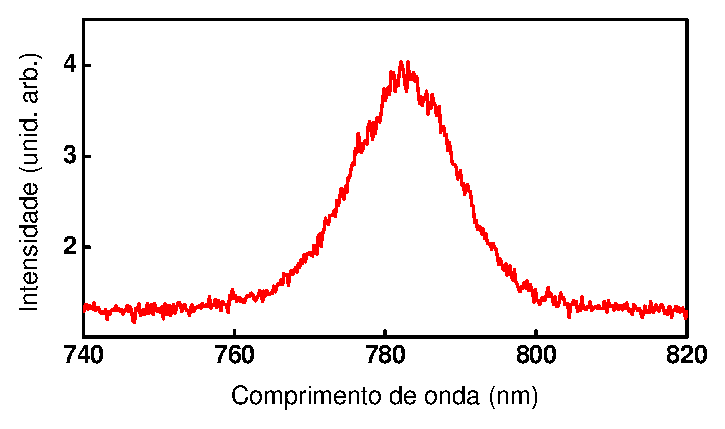
\includegraphics[width=0.6\linewidth]{figuras_do_trabalho/fig1.eps}
	\label{fig2}
	\caption{Espectro de um laser de femtossegundos.}
\end{figure}


%%%%%%%%%%%%%%%%%%%%%%%%%%%%%%%%%%%%%%%%%%%%%%%%%%%%%%%%%%%%%%%
	%%%%%%%%%%%%%%%%%%%%%%%%%%%%%%%%%%%%%%%%%%%%%%%%%%%%%%%%%%%%%%%

\chapter{Conclus�o}

Digite a conclus�o do TCC aqui.


%%%%%%%%%%%%%%%%%%%%%%%%%%%%%%%%%%%%%%%%%%%%%%%%%%%%%%%%%%%%%%%
	%Digite as refer�ncias abaixo
	\bibliography{referencias.bib}
	\bibliographystyle{ieeetr}
	
	
	\backmatter \appendix
%%%%%%%%%%%%%%%%%%%%%%%%%%%%%%%%%%%%%%%%%%%%%%%%%%%%%%%%%%%%%%%
\chapter{T�tulo do Primeiro Ap�ndice}

Digite o primeiro ap�ndice aqui.


%%%%%%%%%%%%%%%%%%%%%%%%%%%%%%%%%%%%%%%%%%%%%%%%%%%%%%%%%%%%%%%
\chapter{T�tulo do Segundo Ap�ndice}
%Para cada ap�ndice adicional, insira o comando \chapter{T�tulo do Ap�ndice}

Digite o segundo ap�ndice aqui.
	
\end{document}